\documentclass[floatfix,reprint,nofootinbib,amsmath,amssymb,epsfig,pre,floats,letterpaper,groupedaffiliation]{revtex4-1}

\usepackage{amsmath}
\usepackage{amssymb}
\usepackage{amsthm}
\usepackage{bm}
\usepackage{dcolumn}
\usepackage[utf8]{inputenc}
\usepackage[ngerman]{babel}
\usepackage{enumitem}
\usepackage{epstopdf}
\usepackage{graphicx}
\usepackage{hyperref}
\usepackage{inconsolata}
\usepackage{listings}
\usepackage{xcolor}
\usepackage{footmisc}

\newcommand{\beq}{\begin{equation}}
\newcommand{\eeq}{\end{equation}}
\newcommand{\e}{\mathrm{e}}
\newcommand{\la}{\langle}
\newcommand{\ra}{\rangle}

\newtheorem{theorem}{Lehrsatz}
\newtheorem{lemma}[theorem]{Hilfssatz}
\newtheorem{assumption}{Annahme}

\theoremstyle{definition}
\newtheorem{observation}{Beobachtung}

\theoremstyle{definition}
\newtheorem{definition}{Definition}

\theoremstyle{definition}
\newtheorem{scenario}{Szenario}

\renewcommand{\andname}{\ignorespaces}
\renewcommand\acknowledgmentsname{Danksagungen}

\makeatletter
\def\Dated@name{Stand: }

\begin{document}

\title{Augur: dezentrales Orakel und Marktvorhersageplattform}

\author{Jack Peterson}
\author{Joseph Krug}
\author{Micah Zoltu}
\author{Austin K. Williams}
\author{und Stephanie Alexander}
\affiliation{Forecast Foundation}

\date{\today}

\begin{abstract}
Augur (zu deutsch ''Prophezeihung'') ist ein vertrauensunabhängiges, dezentrales Orakel und eine Plattform zur Marktvorhersage. Die Ergebnisse von Augurs Prognosemärkten werden durch die Nutzer bestimmt, die Augurs nativen ''Reputation''-Token besitzen und ihre Tokens an prognostizierte Ergebnisse anlegen, wofür sie als Belohnung Durchführungsgebühren der Märkte erhalten. Augurs Anreizstruktur ist so gestaltet, dass ehrliche, akkurate Ergebnisberichte immer die meist-profitabelste Option für Reputation-Tokenhalter ist. Tokenhalter können sich durch Reputationanleihen zusammentun, um vorläufige Marktergebnisse anzufechten. Wenn die Größe der Anleihe eine bestimmte Schwelle erreicht, teilt sich die Reputation in mehrere Versionen, jeweils eine für alle möglichen Marktergebnisse. Tokenhalter müssen nun ihre Reputation-Tokens in eine der Versionen tauschen. Versionen der Reputation, die nicht mit dem Ergebnis der realen Welt zusammenhängen, werden nutzlos, da niemand an Prognosemärkten teilnehmen wird, außer wenn man zuversichtlich ist, dass sich Märkte korrekt auflösen. Demnach werden Tokenhalter nur eine Version der Reputation wählen, die weiterhin ihren Wert behält: nämlich die der Realität entsprechenden Version.
\end{abstract}

\maketitle

Augur ist ein vertrauensunabhängiges, dezentrales Orakel und eine Plattform zur Marktvorhersage. In einem Prognosemarkt können Individuen auf das Ergebnis zukünftiger Ereignisse spekulieren. Diejenigen, die das Ergebnis richtig prognostizieren, erhalten Geld, während diejenigen, die inkorrekte Prognosen stellen, Geld verlieren~\cite{Wolfers_2004, Surowiecki_2005, Hanson_2006}. Der Preis eines Vorhersagemarktes kann als präziser und gut kalkulierter Indikator genutzt werden, wie wahrscheinlich ein Ergebnis eintreffen wird~\cite{Pennock_2001, Manski_2004, Wolfers_2005, Goel_2010}.

Mit der Benutzung von Augur hat man die Möglichkeit, an Prognosemärkten für sehr geringe Gebühren teilzunehmen. Die einzigen signifikanten Ausgaben für Teilnehmer sind die Kompensationen von Marktinitiatoren und Nutzern, die von den Ergebnissen der Märkte berichten, sobald ein Ergebnis eingetreten ist. Das Resultat ist ein Prognosemarkt, in dem Vertrauensbedingungen, Spannungen und Gebühren so niedrig sind, wie sie von konkurrierenden Marktkräften reduziert werden können.

Prognosemärkte sind historisch gesehen zentralisiert. Der einfachste Weg, den Handel in einem Vorhersagenmarkt voranzutreiben, ist ein zentral geführtes Konto bei einem vertrauensvollen Unternehmen. Gleichzeitig ist es am einfachsten, ein Marktergebnis zu bestimmen und die Nutzer auszubezahlen, wenn ein unparteiischer, vertrauensvoller Mediator involviert ist, der Marktergebnisse feststellt. Dennoch birgen zentralisierte Prognosemärkte einige Risiken und Einschränkungen: Sie erlauben keine globale Teilnahme, limitieren die Arten von Märkten, die erstellt und auf denen gehandelt werden kann und sie erfordern das Vertrauen der Händler, Märkte korrekt aufzulösen und nicht deren Geldanlagen zu stehlen.

Augur strebt nach einer vollständig dezentralen Ausführung von Märkten. Dezentralisierte, vertrauensunabhängige Netzwerke wie Bitcoin\cite{Nakamoto_2008} und Ethereum\cite{Buterin_2013} eliminieren die Gefahr, dass Eigeninteressen zu Korruption oder Diebstahl führen. Die einzige Rolle der Augur-Entwickler ist es, Smart Contracts auf dem Ethereum-Netzwerk zu veröffentlichen. Die Augur-Verträge sind vollständig automatisiert: Die Entwickler haben keine Möglichkeit, Gelder auszugeben, die in Verträgen hinterlegt sind, sie kontrollieren keine Marktergebnisse, genehmigen oder lehnen keinen Handel oder anderweitige Transaktionen im Netzwerk ab, können einen Handel nicht rückgängig machen, können keine Bestellungen modifizieren oder stornieren etc. Das Augur-\textit{Orakel} erlaubt es, Informationen der realen Welt auf die Blockchain umzusiedeln, ohne auf eine Zwischeninstanz zu vertrauen. Augur wird das weltweit erste dezentrale Orakel sein.

\section{Wie Augur funktioniert}

Augur-Märkte folgen einer 4-Schritte-Entwicklung: \textit{Erstellung}, \textit{Handel}, \textit{Gutachten} und \textit{Durchführung}. Jeder kann einen Markt auf der Grundlage von Ereignissen in der realen Welt erstellen. Der Handel beginnt sofort nach der Marktveröffentlichung und alle Nutzer können frei auf allen Märkten handeln. Wenn das Event des basierenden Marktes eintritt, wird das Ergebnis des Events vom Augur-Orakel bestimmt. Sobald dies geschehen ist, können Händler ihre Positionen auflösen und Auszahlungen erhalten.

Augur hat einen nativen Token: Reputation (REP). REP wird von Markterstellern und Reportern benötigt, wobei letztere das Ergebnis eines Marktes auf der Augur-Plattform auflösen. Berichterstatter lösen einen Markt durch \textit{Einsatz} seiner REP an einem der möglichen Marktergebnisse auf. Dadurch erklärt der Reporter, dass seiner Anlage das Ergebnis des Marktes zugrundeliegt und dem realen Ausgang entspricht. Der Konsens der Reporter eines Marktes wird als ''Wahrheit'' in Bezug auf das Marktergebnis verstanden. Wenn der Bericht eines Reporters auf das Marktergebnis nicht mit dem Konsens der übrigen Reporter übereinstimmt, verteilt Augur die angelegten REP-Tokens der nicht im Konsens gestimmten Berichterstatter an diejenigen, die das im Konsens ermittelte Ergebnis gewählt haben.

Der Besitz von REP und die Teilnahme an der akkuraten Berichterstattung der Ausgänge von Events berechtigt Tokenhalter an einem Anteil der auf der Plattform eingenommenen Gebühren. Alle angelegten REP-Tokens erlauben den Haltern einen gleichen Anteil an Augurs Marktgebühren. Je mehr REP ein Berichterstatter besitzt und damit korrekt berichtet, umso mehr Gebühren sammelt er für seine Arbeit im Sinne der Plattformsicherheit.

Obwohl REP eine zentrale Rolle in Augurs Betrieb darstellt, wird sie nicht für den Handel genutzt. Händler müssen nie REP besitzen oder nutzen, da sie nicht an der Berichterstattung teilnehmen brauchen.

\begin{figure*}

\includegraphics[width=0.8\textwidth]{overview.pdf}
\caption{Vereinfachte Skizze der Stadien eines Prognosemarktes}
\label{fig:overview}
\end{figure*}

\subsection{Markterstellung}

Augur erlaubt es jedem, einen Markt für bevorstehende Events zu erstellen. Der \textit{Marktersteller} definiert das \textit{Enddatum} eines Events und wählt einen \textit{Reporter}, um das Ergebnis des Events mitzuteilen. Der ernannte Reporter kann nicht eigenmächtig das Ergebnis des Marktes bestimmen. Die Gemeinschaft hat immer die Möglichkeit einzuschreiten und das Ergebnis des Berichterstatters zu korrigieren.

Als nächstes bestimmt der Marktersteller eine \textit{Bezugsquelle}, die Reporter zur Bestimmung des Ergebnisses nutzen sollen. Die Quelle kann lediglich ''Allgemeinwissen'' sein oder aber eine spezifische Quelle wie ''Das Energieinstitut der Vereinigten Staaten'', \texttt{bbc.com} oder die Adresse eines genauen API-Endpunktes\footnote{Wenn z.B. ein Markt für ''Die Temperatur (in Fahrenheit) am 10. April 2018 im internationalen Flughafen von San Francisco, wie von Weather Underground veröffentlicht'' die Bezugsquelle \texttt{https://www.wunderground.com/history/airport/KSFO/2018/4/10/DailyHistory.html} spezifiziert, würden die Reporter einfach die Url ansteuern und die dort angegebene Temperatur in ihrem Bericht angeben.}. Sie bestimmen ebenfalls eine \textit{Erstellungsgebühr}, welche von den Händlern an den Marktinitiator gezahlt wird, welche in den Marktvertrag einwilligen (siehe Abschnitt \ref{section:settlement} bezüglich Gebührendetails). Schließlich definiert der Marktersteller zwei Versicherungen: die \textit{Gültigkeitsversicherung} sowie das  \textit{festgelegte Pfand zum Nicht-Einreichen eines Berichts} (verkürzt als das \textit{Nichtantrittspfand} bezeichnet).

Die Gültigkeitsversicherung wird in ETH bezahlt und dem Marktersteller zurückgeführt, wenn der Markt zu einem anderen Ergebnis als \textit{ungültig} kommt\footnote{Ein \textit{ungültiger Markt} ist ein durch die Reporter bestimmter ungültiger Markt, da kein vom Marktersteller gelistetes Ergebnis korrekt ist oder weil die Wortwahl des Marktes unklar oder subjektiv ist, für Details siehe Abschnitt \ref{section:ambiguous_or_subjective_markets}.}. Die Gültigkeitsversicherung schafft Anreize für Marktinitiatoren, Märkte auf Grundlage von gut definierten Optionen zu erstellen mit objektiven, eindeutigen Ergebnissen. Die Größe der Gültigkeitsversicherung wird dynamisch definiert, basierend auf der Proportion von ungültigen Ergebnissen in neuen Märkten\footnote{Für Details siehe Anhang \ref{section:bond_size_adjustment_details_validity_bonds}}.

Das Nichtantrittspfand besteht aus zwei Teilen: das \textit{Gas-Pfand für den Nichtantritt} (zu zahlen in ETH) sowie das \textit{REP-Pfand für den Nichtantritt} (zu zahlen in REP). Diese Versicherungen werden dem Marktersteller erstattet, wenn der von ihm zugeteilte Reporter innerhalb der ersten drei Tage nach dem \textit{Ereignisenddatum} ein Ergebnis verkündet. Wenn der eingeteilte Reporter seinen Bericht nicht im zugewiesenen 3-Tages-Zeitfenster einreicht, wird der Marktersteller das REP-Pfand für den Nichtantritt verlieren, welches dem \textit{ersten freien Reporter} zufließt, der ein Marktergebnis mitteilt (siehe Abschnitt \ref{section:open_reporting}). Dies lässt den Marktersteller einen verlässlichen Reporter wählen, der bei der schnellen Auflösung von Märkten helfen sollte.

Das Gas-Pfand für den Nichtantritt soll die Gas-Kosten des ersten öffentlichen Reporters decken. Dies vermeidet das Szenario, in dem die Gas-Kosten des ersten öffentlichen Reporters zu hoch sind, um eine Berichterstattung rentabel zu machen. Das Gas-Pfand für den Nichtantritt ist doppelt so hoch wie der durchschnittliche Gas-Preis der Berichterstattung während des vorherigen Gebührenfensters. 

Für den Fall, dass der ausgewählte Reporter kein Ergebnis einreicht, geht das REP-Pfand für den Nichtantritt an den ersten öffentlichen Berichterstatter als Anlage für sein berichtetes Ergebnis über, so dass der erste öffentliche Reporter das REP-Pfand für den Nichtantritt erhält, jedoch nur, wenn er korrekt antwortet. Wie die Gültigkeitsversicherung wird auch das REP-Pfand für den Nichtantritt dynamisch angepasst, basierend auf den Proportionen der zugeteilten Reporter, die nicht rechtzeitig im ersten Gebührenzeitraum geantwortet haben\footnote{Für Details siehe Anhang  \ref{section:bond_size_adjustment_details_no-show_bonds}}.

Der Marktinitiator erstellt den Markt und veröffentlicht alle benötigten Versicherungen durch eine einzelne Ethereum-Transaktion. Sobald die Transaktion bestätigt wurde, ist der Markt aktiv und der Handel beginnt.

\subsection{Handel}

Marktteilnehmer prognostizieren das Ergebnis von Events durch den Handel von \textit{Anteilen} an den Marktergebnissen. Ein \textit{kompletter Satz an Anteilen} ist die Ansammlung von Anteilen, die aus dem Einsatz für jedes mögliche gültige Ergebnis eines Events besteht~\cite{Clark_2014}. Komplette Sätze werden, falls nötig, durch Augurs vertragsgebundenes Treffersystem zum Abschluss des Handels erstellt.

Nehmen wir als Beispiel einen Markt mit zwei möglichen Ergebnissen, \texttt{A} und \texttt{B}. Alice würde 0,7 ETH für einen Anteil an \texttt{A} und Bob würde 0,3 ETH für einen Anteil an \texttt{B} zahlen\footnote{Ursprünglich wird auf Augurs Märkten Ethereums nativer Coin Ether (ETH) zum Handel verwendet. Nachfolgende Versionen von Augur werden auch Märkte mit willkürlichen Ethereum-basierten Tokens unterstützen, inklusive dem Anteil anderer Märkte sowie an Fiat-Währung gebundene Tokens (''stable coins''), falls bzw. wenn diese verfügbar werden}. Zuerst führt Augur diese Bestellungen zusammen und sammelt insgesamt 1 ETH von Alice und Bob\footnote{Die Zahl ''1 ETH'' wird hier zur Vereinfachung gewählt. Die tatsächlichen Kosten eines kompletten Anteilssatzes sind sehr viel kleiner, für Details siehe: \texttt{http://docs.augur.net/\#number-of-ticks}\label{footnote:complete_set_cost}}. Anschließend erstellt Augur einen kompletten Anteilssatz und gibt Alice den Anteil von \texttt{A} und Bob den Anteil von \texttt{B}. So entstehen Anteile an Ergebnissen. Sobald die Anteile erstellt wurden, können sie frei gehandelt werden.

Augurs Handelsverträge pflegen ein Auftragsbuch für jeden Markt auf der Plattform. Man kann jederzeit eine neue Bestellung eingeben oder eine andere füllen. Aufträge werden von einem automatischem Treffersystem gefüllt, das in Augurs Smart Contracts existiert. Anfragen, Anteile zu kaufen oder zu verkaufen, werden sofort ausgeführt, wenn es eine treffende Bestellung bereits im Auftragsbuch gibt. Sie können durch den Kauf von Anteilen an andere Teilnehmer gefüllt werden, die möglicherweise neue komplette Sätze erstellen oder andere bestehende Sätze komplettieren. Augurs Treffersystem beansprucht immer die Mindestmenge an Anteilen und/oder das benötigte Geld, um den Risikowert abzudecken. Wenn es keine treffende Bestellung gibt oder der Auftrag nur teilweise gefüllt werden kann, wird der Rest als neue Bestellung im Auftragsbuch platziert.

Bestellungen werden nie zu einem schlechteren Preis als der des Händlers definierte Limit-Preis ausgeführt, können aber zu einem besseren Preis ausgeführt werden. Ungefüllte und teilweise gefüllte Bestellungen können aus dem Auftragsbuch vom Bestellenden jederzeit entfernt werden. Gebühren werden von Händlern nur bei kompletten Anteilssätzen gezahlt. Durchführungsgebühren werden detailliert in Abschnitt \ref{section:settlement} behandelt.

Auch wenn der Großteil des Anteilshandels erwartungsgemäß vor dem Abschluss des Marktes geschieht, können Anteile jederzeit nach Marktschluss gehandelt werden. Alle Augur-Werte, inklusive den Anteilen an Marktausgängen, Teilnahme-Tokens, Anteilen an einem angefochtenen Pfand und sogar der Besitz eines Marktes selber sind jederzeit transferierbar.

\subsection{Berichterstattung}\label{section:reporting}

Sobald das dem Markt zugrundeliegende Ereignis eintritt, muss das Ergebnis zur Finalisierung und Ausführung eines Marktes bestimmt werden. Ergebnisse werden durch Augurs Orakel festgelegt, welches aus profitmotivierten Reportern besteht, die lediglich das tatsächliche, reale Ergebnis eines Events mitteilen. Jeder, der REP besitzt, kann an der Berichterstattung und Debatte von Ergebnissen teilnehmen. Reporter, deren Berichterstattung mit dem Konsens übereinstimmen, werden finanziell belohnt, während jene, deren Berichterstattung vom Konsens abweicht, finanziell bestraft werden (siehe Abschnitt \ref{section:rep_redistribution}).

\subsubsection{Gebührenzeitraum}

Augurs Berichterstattungssystem findet im Turnus eines \textit{Gebührenzeitraums} von sieben zusammenhängenden Tagen statt. Alle von Augur eingenommenen Gebühren während eines entsprechenden Gebührenzeitraums werden dem \textit{Berichterstattungs-Gebührentopf} des Gebührenfensters hinzugefügt. Zum Ende des Gebührenzeitraums wird die Berichterstattungsgebühr an die REP-Halter ausbezahlt, welche am Berichterstattungsprozess teilgenommen haben. Reporter erhalten eine Belohnung proportional zur im Gebührenzeitraum angelegten Summe von REP. Die Teilnahme beinhaltet: Einsatz während einer initialen Berichterstattung, die Anfechtung eines vorläufigen Ergebnisses oder der Kauf von \textit{Teilnahme-Tokens}.

\subsubsection{Teilnahme-Tokens}

Während eines jeden Gebührenzeitraums können Halter von REP jede Art von Teilnahme-Tokens für jeweils ein Attorep\footnote{Ein \textit{Attorep} ist $10^{-18}$ REP.} kaufen. Am Ende des Gebührenzeitraums können sie ihre Teilnahme-Tokens gegen jeweils ein Attorep eintauschen, zuzüglich eines proportionalen Anteils an den \textit{Berichterstattungs-Gebührentopf} im Gebührenzeitraum. Wenn keine Aktionen des Reporters erforderlich waren (\textit{z.B.} das Einreichen eines Ergebnisses oder Anfechten des Ergebnisses eines anderen Nutzers), kann der Reporter Teilnahme-Tokens kaufen, um zu signalisieren, dass er während des Gebührenzeitraums verfügbar war. Genau wie angelegtes REP können auch Teilnahme-Tokens von ihren Besitzern gegen eine \textit{anteilsmäßige} Gebührenmenge im Gebührenzeitraum eingelöst werden.

Wie in Abschnitt \ref{section:incentives_and_security} beschrieben, ist es wichtig, dass Halter von REP bereit sind, an der Auflösung von Märkten im Falle einer Aufteilung teilzunehmen. Der Teilnahme-Token bietet einen Anreiz für Halter von REP, die Plattform wenigstens einmal pro Woche zu besuchen und im Bedarfsfall bereit für eine Teilnahme zu sein. Halter von REP, die nicht am Berichterstattungsprozess teilnehmen wollen, werden angespornt, wenigstens einmal innerhalb des Gebührenzeitraums von 7 Tagen bei Augur vorbeizuschauen, um Teilnahme-Tokens zu kaufen und Gebühren einzunehmen. Diese beständigen, aktiven Besuche werden sicherstellen, dass sie sich mit der Bedienung Augurs anfreunden, Aufteilungen beachten, falls diese bevorstehen, und vorbereitet sind, an deren Durchführung teilzunehmen.

\subsubsection{Marktstadien}

Augurs Märkte können sich in sieben verschiedenen Stadien nach ihrer Entstehungen befinden. Die potentialen Stadien bzw. ''Phasen'' eines Augur-Marktes sehen wie folgt aus:
\begin{itemize}
\item Ergebnisprognose
\item Zugeteilte Berichterstattung
\item Offene Berichterstattung
\item Wartezeit bis zum nächsten Gebührenzeitraum
\item Streitrunde
\item Aufteilung
\item Abschluss
\end{itemize}

Die Beziehung dieser Stadien kann in Tabelle ~\ref{fig:reporting} eingesehen werden.

\begin{figure*}
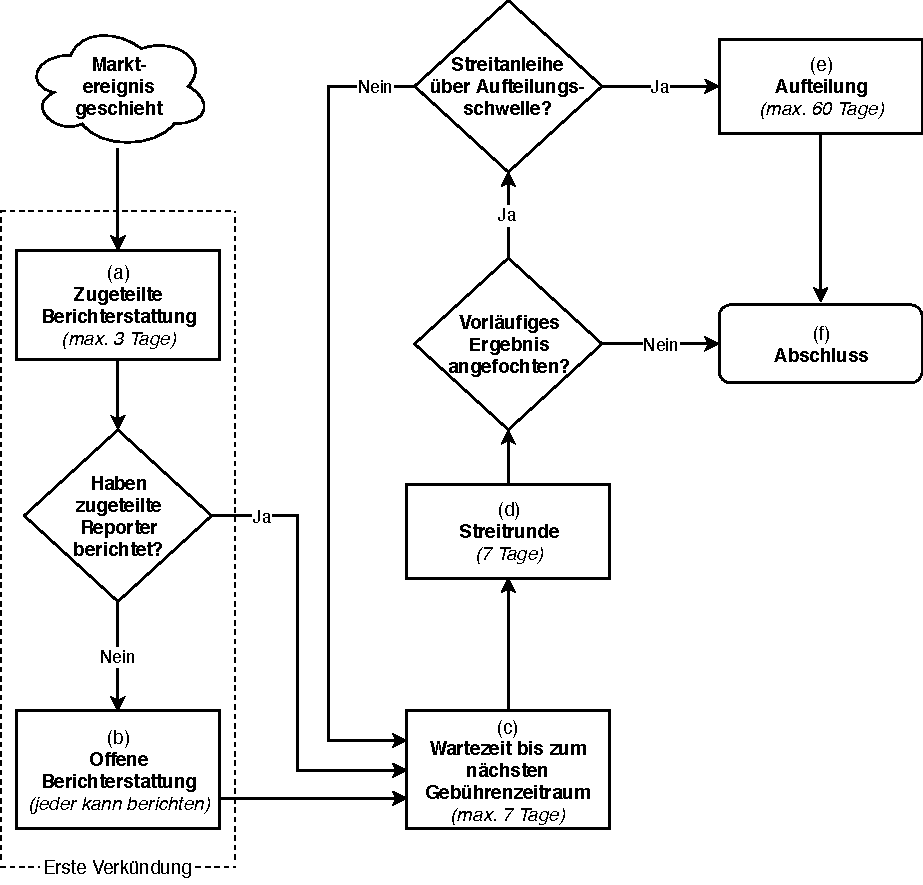
\includegraphics[width=0.8\textwidth]{reporting.pdf}
\caption{Flussdiagramm zur Berichterstattung}
\label{fig:reporting}
\end{figure*}

\subsubsection{Ergebnisprognose}

Die \textit{Ergebnisprognose} oder \textit{Handelsphase} (Diagramm~\ref{fig:overview}) ist der Zeitraum nach dem Handelsstart des Marktes, jedoch bevor das Marktereignis eingetroffen ist. Normalerweise ist dies der handelsaktivste Zeitraum eines jeden Augur-Marktes. Sobald das Ereignisenddatum verstrichen ist, geht der Markt in die \textit{zugeteilte Berichterstattungsphase} über (Diagramm~\ref{fig:reporting}a).

\subsubsection{Zugeteilte Berichterstattung}

Für die Erstellung eines Marktes müssen Marktinitiatoren einen Berichterstatter wählen und ein Nichtantrittspfand freigeben. Während der zugeteilten Berichterstattungsphase (Diagramm~\ref{fig:reporting}a) hat der eingeteilte Reporter bis zu drei Tagen Zeit, das Ergebnis des Events zu verkünden. Wenn er nicht binnen drei Tagen ein Ergebnis einreicht, verliert der Marktersteller sein Nichtantrittspfand und der Markt geht automatisch in die \textit{offene Berichterstattungsphase} über (Diagramm~\ref{fig:reporting}b).

Wenn der zugeteilte Reporter einen Bericht pünktlich einreicht, wird das Nichtantrittspfand an den Marktinitiator zurückgezahlt. Der zugeteilte Berichterstatter muss den Anteil seines angelegten Einsatzes veröffentlichen\footnote{Für Details siehe Anhang \ref{section:bond_size_adjustment_details_designated_reporter_stake} bezüglich der Größe des zugeteilten Reporteranteils}, welcher entfällt, wenn der Markt zu einem anderen Ergebnis als seinem Ergebnis kommt\footnote{Verlorene Anteile werden dem Berichterstattungs-Gebührentopf im entsprechenden Gebührenzeitraum des Marktes hinzugefügt und genutzt, um ehrliche Reporter und Ergebnisanfechter zu belohnen. Für Details siehe Abschnitt \ref{section:rep_redistribution}}. Sobald der zugeteilte Reporter seinen Bericht einreicht, steht der Markt vor der \textit{Wartezeit bis zum nächsten Gebührenzeitraum} (Diagramm~\ref{fig:reporting}c) und das mitgeteilte Ergebnis wird zum \textit{vorläufigen Ergebnis} des Marktes.

\subsubsection{Offene Berichterstattung}\label{section:open_reporting}

Wenn der zugeteilte Reporter nicht während der entsprechenden drei Tage ein Ergebnis verkündet, verliert der Marktinitiator sein Nichtantrittspfand und der Markt wechselt sofort in die \textit{offene Berichterstattung} (Diagramm~\ref{fig:reporting}b). Sobald der Markt in die offene Berichterstattungsphase übergeht, kann jeder den Ausgang eines Marktes verkünden. Wenn der zugeteilte Berichterstatter kein Ergebnis einreicht, wird der erste Berichterstatter, der ein Ergebnis des Marktes verkündet, als \textit{erster öffentlicher Berichterstatter} bezeichnet.

Der erste öffentliche Berichterstatter des Marktes erhält das eingezogene Nichtantrittspfand in Form einer Anlage an dem gewählten Ergebnis, sodass er das REP-Pfand für den Nichtantritt nur beanspruchen kann, wenn sein mitgeteiltes Ergebnis mit dem endgültigen Marktkonsens übereinstimmt. Er erhält das zusätzliche Gas-Pfand für den Nichtantritt erst, wenn der Markt dem verkündeten Ergebnis zustimmt.

Der erste öffentliche Berichterstatter muss \textit{nicht} sein eigenes REP an ein mögliches Ergebnis anlegen, um ein Ergebnis des Marktes zu verkünden. Dadurch sollte das Ergebnis eines Marktes schon bald von \textit{jemand anderem} nach dem Übergang in die offene Berichterstattung verkündet werden, wenn die Ergebnismitteilung durch den zugeteilten Berichterstatter ausgeblieben ist.

Sobald ein \textit{erster Bericht} des anfänglichen Reporters eingeht (sowohl des zugeteilten als auch des ersten öffentlichen Berichterstatters), wird das verkündete Ergebnis zum vorläufigen Marktergebnis und der Markt geht in die Wartezeit bis zum nächsten Gebührenzeitraum über (Diagramm~\ref{fig:reporting}c).

\subsubsection{Wartezeit bis zum nächsten Gebührenzeitraum}

Sobald ein Markt seinen ersten Bericht erhält, beginnt die Wartezeit bis zum nächsten Gebührenzeitraum (Diagramm~\ref{fig:reporting}c). Während dieser Phase werden Marktprognosen bis zum Ende des Gebührenzeitraums ausgesetzt. Sobald der nächste Gebührenzeitraum beginnt, geht der Markt in die \textit{Streitrunde} über.

\subsubsection{Streitrunde}

Die Streitrunde (Diagramm~\ref{fig:reporting}d) besteht aus einem Zeitraum von 7 Tagen, in dem jeder REP-Tokenhalter die Möglichkeit hat, das \textit{vorläufige Marktergebnis} anzufechten\footnote{Der Umstand, dass die Streitrunden in die Gebührenzeiträume fallen, ist reine Annehmlichkeit. Grundsätzlich können Streitrunden und Gebührenzeiträume unterschiedlich sein.}. (Zu Beginn einer Streitrunde ist ein vorläufiges Marktergebnis das Ergebnis, das zum finalen Resultat führt, sofern es nicht erfolgreich von REP-Haltern angefochten wird.) Eine Streitrunde besteht aus dem \textit{Einsatz} von REP (in diesem Kontext als \textit{Streiteinsatz} bezeichnet) auf ein \textit{anderes} Ergebnis als das vorläufige Marktergebnis. Ein Streitrunde ist \textit{erfolgreich}, wenn die gesamte Menge des Streiteinsatzes für ein Ergebnis die \textit{Streitanleihengröße} erreicht, die für die aktuelle Runde benötigt wird. Die Streitanleihengröße wird wie folgt berechnet:

Lassen wir $A_n$ den Gesamteinsatz für alle möglichen Marktausgänge zu Beginn einer Streitrunde $n$ sein. $\omega$ kann ein beliebiges Marktergebnis sein, jedoch \textit{anders als} das vorläufige Marktergebnis zu Beginn dieser Streitrunde. Dann bezeichnet $S(\omega, n)$ den Gesamteinsatz eines Ergebnisses $\omega$ zu Beginn einer Streitrunde $n$. Somit wird die Größe des \textit{Streiteinsatzes} benötigt, um erfolgreich das vorläufige Ergebnis für ein neues Resultat $\omega$ anzufechten, wobei Runde $n$ durch $B(\omega, n)$ dargestellt wird und sich wie folgt zusammensetzt:
\beq \label{eq:bond_size}
B(\omega, n) = 2A_n - 3S(\omega, n)
\eeq

Die Pfandgrößen werden in dieser Weise berechnet, um eine genaue Einsatzrendite von 50\% für Berichterstatter festzulegen, die erfolgreich falsche Ergebnisse anfechten (siehe Abschnitt \ref{section:leveraging_the_threat_of_a_fork}).

Ein Streiteinsatz muss gänzlich von einem einzigen Nutzer gezahlt werden. Die Augur-Plattform erlaubt es Teilnehmern, eine Streitanleihe durch Crowdsourcing zu sammeln. Jeder Nutzer, der ein inkorrektes vorläufiges Ergebnis sieht, kann es durch Einsatz seiner REP zugunsten eines anderen Ergebnisses anfechten. Falls ein anderes Ergebnis als das vorläufige Ergebnis einen ausreichenden Streiteinsatz erhält, um seine Streitanleihe zu decken, wird das derzeitige vorläufige Ergebnis erfolgreich angefochten.

Im Falle einer erfolgreichen Streitrunde wird der Markt entweder in eine weitere Streitrunde gehen oder ins Stadium der \textit{Aufteilung} wechseln (Diagramm~\ref{fig:reporting}e). Wenn die Größe des gesammelten Streiteinsatzes größer als 2.5\% aller REP ist, wird der Markt ins Aufteilungsstadium übergehen. Wenn die Größe des gesammelten Streiteinsatzes kleiner als 2.5\% aller REP ist, wird das neugewählte Ergebnis das neue vorläufige Ergebnis des Marktes und der Markt geht in eine neue Streitrunde über.

Sämtlicher Streiteinsatz wird treuhänderisch während der Streitrunde verwaltet. Wenn ein Streiteinsatz nicht erfolgreich war, wird er am Ende der Streitrunde an seine Besitzer zurückgegeben. Wenn keine Anfechtung innerhalb der siebentägigen Streitrunde erfolgreich ist, geht der Markt ins \textit{Abschlussstadium} über (Diagramm~\ref{fig:reporting}f) und sein vorläufiges Ergebnis wird als \textit{endgültiges Ergebnis} angenommen. Das endgültige Ergebnis eines Marktes ist das vorläufige Ergebnis, das eine Streitrunde durchläuft ohne erfolgreich angefochten worden zu sein oder durch eine Aufteilung bestimmt wird. Augurs Verträge behandeln endgültige Ergebnisse als \textit{Wahrheit} und nehmen dementsprechend Auszahlungen vor.

Jeglicher nicht erfolgreich angelegter Streiteinsatz wird an die ursprünglichen Anleger nach Beendigung einer jeden Streitrunde zurückerstattet. Jeder erfolgreiche Streiteinsatz wird dem durchgesetzten Ergebnis zugeführt und verbleibt dort bis zum Abschluss des Marktes (oder bis eine Aufteilung in einem anderen Augur-Markt erfolgt). Jeder Streiteinsatz (ob erfolgreich oder nicht) wird ein Teil des \textit{Berichterstattungs-Gebührentopfs}\footnote{Alle Durchführungsgebühren und Gültigkeitsversicherungen, die während eines Gebührenzeitraums eingenommen werden, werden dem Berichterstattungs-Gebührentopf während des Gebührenzeitraums hinzugefügt. Zum Ende des Gebührenzeitraums wird der Berichterstattungs-Gebührentopf an die Benutzer ausgezahlt in Proportion zur Menge an REP, die sie während des Gebührenzeitraums angelegt haben.} während des Gebührenzeitraums erhalten.

\subsubsection{Aufteilung}\label{section:fork}

Das Aufteilungsstadium (Diagramm~\ref{fig:reporting}e) ist ein spezielles Stadium, welches bis zu 60 Tage andauern kann. Eine Aufteilung ist die letztmögliche Option, um einen Markt aufzulösen. Es ist ein sehr störender Prozess und sollte auch nur selten auftreten. Eine Aufteilung entsteht, wenn es einen Markt mit einem Ergebnis durch den erfolgreich gesammelten Streiteinsatz von mindestens 2.5\% aller REP gibt. Dieser Markt wird als \textit{aufgeteilter Markt} bezeichnet.

Wenn eine Aufteilung initiiert wurde, beginnt ein 60-tägiger\footnote{Ein Aufteilungszeitraum kann kürzer als 60 Tage sein: Ein Aufteilungszeitraum endet, wenn entweder 60 Tage verstrichen sind oder mehr als 50\% aller ursprünglichen REP in ein Folgeuniversum gewechselt sind.} \textit{Aufteilungszeitraum}. Die Anfechtung aller anderen nicht abgeschlossenen Märkte wird bis zum Ende des Aufteilungszeitraums ausgesetzt. Der Aufteilungszeitraum ist um einiges länger als der gewöhnliche Gebührenzeitraum, da die Plattform den REP-Haltern und Serviceanbietern (wie Wallets und Börsen) genügend Zeit einräumen muss, um sich vorzubereiten. Das Ergebnis einer Aufteilung kann nicht angefochten werden.

Jeder Augur-Markt und alle REP-Tokens existieren in einem \textit{Universum}. REP-Tokens können genutzt werden, um ein Ergebnis zu verkünden (und dadurch Gebühren einzunehmen), jedoch \textit{nur} für Märkte, die im gleichen Universum wie die REP-Tokens existieren. Wenn Augur veröffentlicht wird, existieren alle Märkte und REP zusammen im gleichen \textit{Ursprungsuniversum}.

Wenn sich ein Markt teilt, werden neue Universen erschaffen. Aufteilung erschafft ein \textit{Folgeuniversum} für jedes mögliche Ergebnis des aufteilenden Marktes (inklusive \texttt{ungültiger} Ergebnisse, wie in Abschnitt \ref{section:settlement_of_invalid_markets} beschrieben). Beispielsweise hat ein ''zweigeteilter'' Markt drei mögliche Resultate: \texttt{A}, \texttt{B} und \texttt{ungültig}. Von daher wird ein zweiteilender Markt drei neue Folgeuniversen erschaffen: Universum \texttt{A}, Universum \texttt{B} und Universum \texttt{ungültig}. Diese drei neuen Universen sind zunächst leer: sie beinhalten keine Märkte oder REP-Tokens.

Wenn eine Aufteilung durchgeführt wird, wird das \textit{Altuniversum} permanent \textit{geschlossen}. In einem geschlossenen Universum können keine neuen Märkte erstellt werden. Nutzer können weiterhin Anteile in geschlossenen Universen handeln und Märkte in einem geschlossenen Universum können immer noch Berichterstattungen erhalten. Jedoch werden dort keine Berichterstattungs-Belohnungen mehr ausgeschüttet und Märkte in geschlossenen Universen können nicht mehr abgeschlossen werden. Damit Märkte oder REP-Tokens in jenen Universen weiterhin nützlich bleiben, müssen sie erst in ein Folgeuniversum umziehen.

Halter von REP-Tokens im Altuniversum können mit ihren Tokens in ein Folgeuniversum ihrer Wahl umziehen. Die Wahl sollte sorgfältig erfolgen, da die Migration nur in eine Richtung funktioniert und nicht reversibel ist. Tokens können nicht von einem Folgeuniversum zu einem anderen gesendet werden. \textit{Migration ist eine dauerhafte Zusage von REP-Tokens an ein spezielles Marktergebnis.} REP-Tokens, die in verschiedene Folgeuniversen umziehen, sollten als gänzlich separate Tokens angesehen werden und Diensteanbieter wie Wallets und Handelsplattformen müssen sie auch dementsprechend behandeln.

Wenn eine Aufteilung initiiert wurde, ist jegliche REP \textit{ungebunden}, das an nicht aufteilenden Märkten angelegt ist, sodass es frei in ein Folgeuniversum während des Aufteilungszeitraums umziehen kann\footnote{Die einzige Ausnahme ist die angelegte REP des ersten Berichterstatters, wenn er das erste Ergebnis erstellt hat. Diese REP bleibt an das erste verkündete Ergebnis gebunden und migriert automatisch in das Folgeuniversum, das die Aufteilung gewinnt.}.

Das Folgeuniversum, das die meiste migrierte REP am Ende der Aufteilungsphase erhält, wird zum \textit{gewinnenden Universum} und sein zugehöriges Ergebnis wird zum endgültigen Ergebnis des geteilten Marktes. Unabgeschlossene Märkte im Altuniversum können nur in das gewinnende Universum umziehen und werden, wenn sie ein erstes Ergebnis erhalten haben, in das Wartezeit-Stadium für den nächsten Gebührenzeitraum zurückgesetzt.

\paragraph*{Es gibt kein Zeitlimit, um mit Tokens aus dem Altuniversum in ein Folgeuniversum umzuziehen.} Tokens können nach der Aufteilungsphase umziehen, haben jedoch keinen Einfluss mehr auf das gewinnende Universum. Um eine größere Teilnahme während des Aufteilungszeitraums zu erreichen, erhalten alle Tokenhalter, die binnen 60 Tagen mit ihrer REP umziehen, zusätzlich 5\% an REP im Folgeuniversum, in das sie migrieren\footnote{Dies gilt auch dann, wenn die Aufteilungsphase früher endet, da mehr als 50\% aller REP in ein Folgeuniversum transferiert wurde.}. Diese Belohnung wird durch die Prägung neuer REP-Tokens erzielt\footnote{Die Auswirkung dieser Addition auf die Geldmenge ist minimal. Zum Beispiel, wenn 20\% der existierenden REP während einem Aufteilungszeitraum einer Aufteilung umziehen, würde dieser Bonus zu einer 1\%igen Steigerung des Geldbetrags von REP führen. Darüber hinaus werden Aufteilungen als sehr seltene Ereignisse angesehen.}.

\paragraph*{Berichterstatter, die ihre REP an einem der Marktergebnisse angelegt haben, können ihre Position nicht während der Aufteilung ändern.} REP, die an einem Ergebnis im Altuniversum angelegt wurde, kann nur in ein korrespondierendes Folgeuniversum umziehen. Wenn beispielsweise ein Berichterstatter geholfen hat, den erfolgreichen Streiteinsatz zugunsten Ausgang \texttt{A} während einer Streitrunde zu sammeln, kann die von ihnen angelegte REP am Ergebnis \texttt{A} auch nur in Universum \texttt{A} während der Aufteilung umziehen.

\paragraph*{Folgeuniversen sind komplett getrennt.} REP-Tokens, die in einem Universum existieren, können nicht für die Berichterstattung von Events oder für den Verdienst aus Märkten eines anderen Universums genutzt werden. Da Nutzer vermutlich keine Märkte erstellen oder darauf handeln wollen, dessen Orakel nicht vertrauenswürdig ist, wird REP in einem Universum, das nicht mit der objektiven Realität korrespondiert, nur unwahrscheinlich seinem Besitzer Gebühren einbringen und somit keinen signifikanten Marktwert haben. Von daher sollten REP-Tokens, die in ein Universum umgezogen sind, das keinen objektiven Wahrheitsbezug herstellt, keinen Marktwert haben, unabhängig davon, ob das falsche Universum eine Aufteilung gewinnt oder nicht. Dies hat wichtige Konsequenzen für die Sicherheit, welche wir in Abschnitt \ref{section:incentives_and_security} behandeln.

\subsubsection{Abschluss}

Ein Markt wechselt ins Abschlussstadium (Diagramm~\ref{fig:reporting}f), wenn es eine siebentägige Streitrunde durchlaufen hat, ohne, dass sein vorläufiges Ergebnis angefochten wurde, oder nach der Durchführung einer Aufteilung. Das Resultat einer Aufteilung kann nicht angefochten werden und wird immer als abgeschlossen am Ende der Aufteilungsphase angesehen. Sobald ein Markt abgeschlossen ist, können Händler ihre Positionen direkt mit dem Markt auswerten. Wenn ein Markt den abgeschlossenen Status erreicht, nennen wir das gewählte Ergebnis \textit{endgültiges Ergebnis}.

\subsection{Marktausführung}\label{section:settlement}

Ein Händler kann seine Position in einer von zwei Weisen abschließen: durch Verkauf der Anteile an einen anderen Händler im Tausch einer Währung oder durch Abgleich seiner Anteile mit dem Markt. Zur Erinnerung: Jeder Anteil existiert erst als Teil eines kompletten Satzes, wenn insgesamt 1 ETH von Augur verwaltet wurde\footref{footnote:complete_set_cost}. Um 1 ETH aus der Verwaltung zurückzuerhalten, müssen Händler an Augur entweder einen Satz oder, wenn der Markt abgeschlossen wurde, einen Anteil ihres Gewinns abgeben. Wenn dieser Austausch stattfindet, nennen wir ihn die \textit{Ausführung des Marktvertrags} durch den Nutzer.

Betrachten wir beispielsweise einen nicht abgeschlossenen Markt mit den möglichen Ergebnissen \texttt{A} und \texttt{B}. Wir sagen, dass hat Alice einen Anteil am Ergebnis \texttt{A} hat, den sie für 0,7 ETH verkaufen möchte. Bob hat einen Anteil am Ergebnis \texttt{B}, das er für 0,3 ETH verkaufen will. Als erstes führt Augur die Bestellungen zusammen und nimmt die Anteile \texttt{A} und \texttt{B} von den Teilnehmern. Dann gibt Augur 0,7 ETH (abzüglich Gebühren) an Alice und 0,3 ETH (abzüglich Gebühren) an Bob.

Als zweites Beispiel betrachten wir einen abgeschlossenen Markt, in dem sich Ergebnis \texttt{A} durchsetzt. Alice hat einen Anteil an \texttt{A} und will diesen einlösen. Sie sendet ihren Anteil von \texttt{A} an Augur und erhält 1 ETH (abzüglich Gebühren) zurück.

\subsubsection{Ausführungsgebühren}

Der einzige Zeitpunkt, an dem Augur Gebühren erhebt, ist, wenn Marktteilnehmer gemäß Marktvertrag abrechnen. Augur erhebt zwei Gebühren während der Ausführung: die Erstellungsgebühr und die Berichterstattungsgebühr. Beide Gebühren sind proportional zur ausgezahlten Menge. Demnach würden im Beispiel oben vor der Ausführung, bei der Alice 0,7 ETH und Bob 0,3 ETH erhält, Alice 70\% und Bob 30\% der Gebühren zahlen.

Die Markterstellungsgebühr wird vom Marktinitiator während der Markterstellung festgelegt und beim Marktabschluss an ihn bezahlt. Die Berichterstattungsgebühr wird dynamisch berechnet (siehe Abschnitt \ref{section:market_cap_nudges}) und an die Reporter gezahlt, die an der Berichterstattung teilnehmen.

\subsubsection{Ausführung ungültiger Märkte}\label{section:settlement_of_invalid_markets}

Wenn sich ein Markt als \texttt{ungültig} auflöst, erhalten gemäß dem Marktvertrag abschließende Händler den gleichen Betrag an ETH gemäß ihrer Anteile am Ergebnis. Wenn der Markt $N$ mögliche Ergebnisse hatte (abzüglich des \texttt{ungültigen} Ergebnisses) und die Kosten eines kompletten Anteilssatzes $C$ ETH waren, erhalten Händler $C/N$ ETH für jeden Anteil nach Marktvertrag\footnote{Ein Handel kann nicht einfach ausgeführt werden, wenn sich ein Markt als \texttt{ungültig} aufgrund technischer Limitierungen erweist. Anteile an Ergebnissen sind lediglich Tokens, die direkt zwischen Nutzern gehandelt werden können. Das ETH und Anteile stehen daher nicht unter Augurs Kontrolle und können nicht an den ursprünglichen Besitzer zurückgegeben werden, wenn ein Markt als \texttt{ungültig} geschlossen wird.}.

\subsubsection{Rückverteilung der Reputation}\label{section:rep_redistribution}

Wenn ein Markt ohne eine Aufteilung abschließt, ist jede REP, die an ein beliebiges Ergebnis außer dem endgültigen Marktergebnis angelegt wurde, verwirkt und wird an die Nutzer verteilt, die am endgültigen Marktergebnis angelegt haben in Proportion zur Menge ihrer angelegten REP. Die Streitanleihengröße wird so bemessen, dass jeder, der erfolgreich ein Ergebnis im Sinne des endgültigen Marktergebnisses anfechtet, mit 50\% seines Investments als Streiteinsatz belohnt wird\footnote{Siehe Leitsatz \ref{th:roi_guarantee} in Anhang \ref{section:finalization_time}.}. Dies ist ein starker Anreiz für Reporter, falsche vorläufige Ergebnisse anzufechten.

\section{Anreize und Sicherheit}\label{section:incentives_and_security}

Es gibt einen engen Zusammenhang zwischen dem Marktwert von REP und der Vertrauenswürdigkeit von Augurs Aufteilungsprotokoll. Wenn der Marktwert von REP groß genug ist\footnote{Für Details siehe Abschnitt \ref{section:integrity_forking_protocol}} und Angreifer wirtschaftlich gesehen vernünftig agieren, sollte das Ergebnis, welches die Aufteilung gewinnt, mit der objektiven Realität übereinstimmen. Es wäre für Augur sogar möglich, problemlos ohne zugeteilte Berichterstatter und Streitrunden zu funktionieren. Durch die \textit{alleinige} Wahl des Aufteilungsprozesses würde das Orakel wahrheitsgetreu berichten.

Allerdings sind Aufteilungen störend und zeitintensiv. Eine Marktaufteilung dauert bis zu 60 Tage und kann lediglich einen Markt zur gleichen Zeit auflösen. Während der 60 Tage, in denen die Marktaufteilung durchgeführt wird, werden alle anderen nicht abgeschlossenen Märkte ausgesetzt\footnote{Händler können weiterhin auf diesen Märkten handeln, jedoch können diese Märkte nicht vor dem Abschluss des Aufteilungsprozesses aufgelöst werden.}. Diensteanbieter müssen sich aktualisieren und REP-Halter müssen ihre REP zu einer der Folgeuniversen migrieren. Von daher sollten Aufteilungen nur genutzt werden, wenn sie absolut notwendig sind. Eine Aufteilung ist die nukleare Option.

Sobald man sich einig ist, dass einer Aufteilung für die Wahrheitsfindung vertraut werden kann, können Anreize genutzt werden, um Teilnehmer zu ermutigen, sich ehrlich zu verhalten ohne eine Aufteilung zu initiieren. \textit{Es sind die zuverlässige Gefahr einer Aufteilung und der Glaube, dass sich die Aufteilung richtig auflösen wird, die die Eckpfeiler von Augurs Anreizprogramm darstellen.}

Als nächstes betrachten wir die Konditionen, bei denen dem Aufteilungssystem vertraut werden kann, um die Wahrheit zu ermitteln. Anschließend  diskutieren wir das Anreizprogramm und wie es zur schnellen und korrekten Auflösung von Märkten anregt.

\subsection{Integrität des Aufteilungsprotokolls}\label{section:integrity_forking_protocol}

Hier gehen wir auf die Verlässlichkeit des Aufteilungsprozesses ein und auf die Konditionen, unter denen ihm vertraut werden kann. Wenn wir auf eine Aufteilung verweisen, nehmen wir der Einfachheit halber Bezug auf das Folgeuniversum, das mit dem tatsächlichen Ergebnis als \texttt{wahres} Universum korrespondiert, sowie jeglichem anderen Folgeuniversum als \texttt{falsches} Universum. Wir werden auf das Folgeuniversum Bezug nehmen, welches die meiste REP während des Umzugs in der Aufteilungsphase erhält und somit zum gewinnenden Universum wird, während alle anderen Folgeuniversen verlieren.

Naturgemäß wollen wir immer nur das \texttt{wahre} Universum als gewinnendes Universum sehen und die \texttt{falschen} Universen als verlierende Universen. Wir sagen, dass das Aufteilungsprotokoll dann erfolgreich gehackt wurde, wann immer ein \texttt{falsches} Universum das gewinnende Universum einer Aufteilung ist und somit der resultierende, sich aufteilende Markt (und potentiell auch alle unabgeschlossenen Märkte) falsch ausgezahlt werden.

Der Ansatz, das Orakel zu sichern, ist die Einrichtung von Maßnahmen wie ein maximaler Ertrag eines erfolgreichen Angreifers, der kleiner als die minimalen Kosten einer Attacke ausfällt. Wir formulieren dies nachstehend.

\subsubsection{Maximaler Ertrag eines Angreifers}

Ein Angreifer, der erfolgreich das Orakel attackiert, würde alle unabgeschlossenen Augur-Märkte zwingen, zu einem \texttt{falschen} Universum zu migrieren. Wenn der Angreifer die Mehrheit der REP im \texttt{falschen} Universum hält, kann der Angreifer alle unabgeschlossenen Märkte zwingen, sich so aufzulösen, wie er es möchte. Im extremsten Fall wäre er auch fähig, alle hinterlegten Gelder aller Märkten einzunehmen\footnote{Dies erfordert, dass der Angreifer \textit{alle} Anteile eines möglichen Ergebnisses abgreift und dann den Markt zwingt, mit diesem Ergebnis abzuschließen.}.

\begin{definition}
Wir definieren und kennzeichnen mit $I_a$ Augurs \textit{natives offenes Interesse} als den Wert der Summe aller hinterlegten Werte in unabgeschlossenen Augur-Märkten\footnote{Dies beinhaltet externe Märkte, die Berichterstattungsgebühren an Augur zahlen.}.
\end{definition}

\begin{definition}
Wir definieren einen \textit{störenden Markt} als jeden Markt, der keine Berichterstattungsgebühren an Augur zahlt, sich jedoch gemäß dem Abschluss eines nativen Augur-Marktes auflöst.
\end{definition}

\begin{definition}
Wir definieren und kennzeichnen mit $I_p$ das \textit{schadhafte öffentliche Interesse} als den Wert der Summe aller hinterlegten Werte in einem schadhaften Markt, der sich gemäß eines nicht abgeschlossenen, nativen Augur-Marktes auflöst.
\end{definition}

Im extremsten Fall wäre ein Angreifer auch fähig, alle Werte in allen schadhaften Märkten abzugreifen, die sich gemäß unabgeschlossener, nativer Augur-Märkte auflösen.

\begin{observation}
Der maximale Gesamtnutzen für einen Angreifer, der erfolgreich das Orakel attackiert, ist $I_a + I_p$.
\end{observation}

\subsubsection{Schadhaftes, öffentliches Interesse ist nicht zu ahnen}

Augur kann akkurat und effizient $I_a$ bemessen. Dennoch kann $I_p$ nicht allgemein erkannt werden, da willkürlich viele schadhafte Offline-Märkte existieren können, jeder mit willkürlich großem, öffentlichem Interesse. Da der maximal mögliche Nutzen eines Angreifers die unbekannte Menge $I_p$ beinhaltet, kann man nie objektiv sicher sein, dass das Orakel sicher gegen wirtschaftlich vernünftige Angreifer ist.

Dennoch wollen wir annehmen, dass $I_p$ in der Praxis ausreichend gebunden ist und Bedingungen definieren, unter denen wir bestätigen können, dass das Orakel sicher ist.

\subsubsection{Minimale Kosten einer schadhaften Attacke}

Als nächstes betrachten wir die Kosten einer Attacke auf das Orakel. $P$ soll den Preis der REP kennzeichnen. $\epsilon$ repräsentiert ein Attorep\footnote{Ein \textit{Attorep} ist $10^{-18}$ REP.}. $M$ kennzeichnet die ingesamt existierende Summe von REP (die ''Geldmenge'' von REP). $S$ zeigt den Anteil von $M$, der ins wahre Universum während der Aufteilungsphase einer Aufteilung migriert.

Von daher symbolisiert das Produkt $SM$ die absolute Summe an REP, die ins wahre Universum in der Aufteilungsphase einer Aufteilung umzieht, wobei das Produkt $PM$ der Marktwert von REP ist.

$P_f$ soll den Preis der REP darstellen, die in ein \texttt{falsches}, vom Angreifer gewähltes Universum transferiert wurde. Es gilt zu beachten, dass wenn $P \leq P_f$ ist, das Orakel nicht sicher gegen wirtschaftlich vernünftige Angreifer wäre, da es mindestens genauso profitabel ist, REP ins falsche Universum zu migrieren, wie es gar nicht zu migrieren.

\subsubsection{Integrität}

\begin{assumption}
Berichterstatter, die keine Angreifer sind, werden nie REP in ein \texttt{falsches} Universum bei einer Aufteilung transferieren\footnote{Es mag Fälle geben, in denen manche unschädliche Reporter ihre REP zufällig oder fahrlässig in ein \texttt{falsches} Universum transferieren. Ein solches Verhalten ist in der Praxis nicht von der Kollaboration mit einem Angreifer zu unterscheiden.}.
\end{assumption}

Für eine erfolgreiche Attacke auf das Orakel bedarf es absichtlich einer größeren Migration von REP in ein \texttt{falsches} Universum, als in das \texttt{wahre} Universum während der Aufteilungsphase einer Aufteilung. Nur der Angreifer wird vermutlich REP in ein \texttt{falsches} Universum transferieren. Die Menge an REP, die in das \texttt{wahre} Universum während der Aufteilungsphase transferiert wird, wird als $SM$ dargestellt. Von daher muss ein Angreifer, um erfolgreich zu sein, mindestens $SM + \epsilon$ REP migrieren. Zur Einfachheit werden wir das vernachlässigbare $\epsilon$ ignorieren und annehmen, dass eine erfolgreiche Attacke eine Migration von mindestens $SM$ REP voraussetzt, was einen Wert von $SMP$ vor dem Transfer in ein \texttt{falsches} Universum bedeutet.

Wenn ein Angreifer $SM$ REP während der Aufteilungsphase einer Aufteilung migriert, wird er $SM$ REP im Folgeuniversum erhalten, in das er umzieht\footnote{Konkret würde der Angreifer $1,05 SM$ REP im Folgeuniversum erhalten, aufgrund des 5\%-Bonus für die Migration binnen 60 Tagen ab Beginn der Aufteilung. Wir ignorieren den 5\%-Bonus an dieser Stelle für die Einfachheit der Diskussion. Um eine Diskussion einschließlich des 5\%-Bonus' zu sehen, beachten Sie Anhang \ref{ap:early_migration_integrity}.}. Wenn der Angreifer in ein \texttt{falsches} Universum migriert, wird der Wert der Coins $SMP_f$ betragen. Somit sind die minimalen Kosten für einen Angreifer $(P - P_f)SM$.

\begin{observation}
Die minimale Summe an REP, die ein erfolgreicher Angreifer in ein \texttt{falsches} Universum während der Aufteilung migrieren muss, ist $SM$, was den Angreifer $(P - P_f)SM$ kostet.
\end{observation}

Beachten Sie, dass wenn $S > \frac{1}{2}$ ist, eine Attacke \textit{unmöglich} wäre, da nicht genügend REP außerhalb des \texttt{wahren} Universums existiert, sodass ein \texttt{falsches} Universum das gewinnende Universum würde.

Entgegen wirtschaftlich vernünftigen Angreifern wird das Orakel zu Ergebnissen kommen, die mit der objektiven Realität übereinstimmen, wenn der maximale Nutzen eines Angreifers geringer als die minimalen Kosten einer Attacke ausfallen. In den Beobachtungen 1 \& 2 können wir sehen, dass dies immer eintritt, wenn $S > \frac{1}{2}$ oder $I_a + I_p < (P - P_f)SM$ ist. Das erlaubt uns unsere formale Definition von Integrität.

\begin{definition}\label{ob:integrity_property}
(Integritätsbestätigung) Das Aufteilungsprotokoll hat immer dann \textit{Integrität}, wenn $S > \frac{1}{2}$ oder wenn $I_a + I_p < (P - P_f)SM$ ist.
\end{definition}

Die obige Ungleichheit kann durch $PM$ gelöst werden, um den Zusammenhang zwischen der Integrität des Aufteilungsprotokolls und dem Marktwert von REP herzustellen.

\begin{theorem}\label{th:market_cap_security_theorem}
(Sicherheitsleitsatz für den Marktwert) Das Aufteilungsprotokoll hat nur dann Integrität, wenn:
\begin{enumerate}
\item $S > \frac{1}{2}$ oder
\item $P_f < P$ und der Marktwert von REP größer als $\frac{(I_a + I_p)P}{(P - P_f)S}$ ist.
\end{enumerate}
\end{theorem}

\begin{proof}
Angenommen das Aufteilungsprotokoll besitzt Integrität, dann ist definitionsgemäß $S > \frac{1}{2}$ oder $I_a + I_p < (P - P_f)SM$. Angenommen $I_a + I_p < (P - P_f)SM$. Da $I_a + I_p \geq 0$ und $SM > 0$ sind, wissen wir, dass $P_f < P$ ist. Beim Lösen von $I_a + I_p < (P - P_f)SM$ für $PM$ sehen wir also, dass $\frac{(I_a + I_p)P}{(P - P_f)S} < PM$ ist. Dadurch ist die erste Richtung geprüft.

Jetzt nehmen wir an, dass $S > \frac{1}{2}$ ist oder $P_f < P$ und $\frac{(I_a + I_p)P}{(P - P_f)S} < PM$ ist. Wenn $S > \frac{1}{2}$ ist, besitzt das Aufteilungsprotokoll erklärtermaßen Integrität. Wenn $P_f < P$ und $\frac{(I_a + I_p)P}{(P - P_f)S} < PM$ ist, dann, dann stellen wir bei der Lösung der Ungleichheit für $I_a + I_p$ fest, dass $I_a + I_p < (P-P_f) SM$ ist und das Aufteilungsprotokoll Integrität besitzt.
\end{proof}

\subsection{Unsere Annahmen und ihre Konsequenzen}

Wir glauben, dass Händler nicht auf Augur in einem Universum handeln wollen, in dem Berichterstatter gelogen haben. Wir glauben ebenfalls, dass Marktersteller nicht für das Erstellen von Augur-Märkten in einem Universum zahlen werden, in dem kein Handel stattfindet. In einem Universum ohne Märkte oder Handel erlaubt REP keine Dividenden an diejenigen, die es anlegen. Von daher glauben wir, dass an ein \texttt{falsches} Universum gesendete REP einen belanglosen Marktwert haben und modellieren dies mit $P_f = 0$.

Wir denken, es ist realistisch zu erwarten, dass wenigstens 20\% der existierenden REP während der Aufteilungsphase einer Aufteilung dem wahren Ergebnis zukommen und modellieren dies als $S \geq \frac{1}{5}$. Wir wollen außerdem schadhaftes, öffentliches Interesse von 50\% des ursprünglichen öffentlichen Interesses unterbringen und nehmen daher $I_a \geq 2 I_p$ an.

Unter diesen Umständen erklärt uns Leitsatz \ref{th:market_cap_security_theorem}, dass das Aufteilungsprotokoll Vollständigkeit besitzt, wann immer der Marktwert von REP wenigstens 7,5-mal dem ursprünglichen öffentlichen Interesse ist\footnote{Siehe Anhang \ref{section:alternative_assumptions} für weitere alternative Annahmen und ihre Konsequenzen.}.

\subsection{Anhebung des Marktwerts}\label{section:market_cap_nudges}

Augur bezieht Informationen über den Preis von REP in gleicher Weise wie es alle anderen Informationen über die reale Welt erhält: durch einen Augur-Markt. Dies gibt Augur die Fähigkeit, den aktuellen Marktwert von REP zu berechnen. Augur kann ebenfalls das derzeitige öffentliche Interesse messen und dadurch absehen, was der Marktwert sein müsste, um Augurs Integritätsbedingungen zu erfüllen.

Jedes Universum beginnt mit einer standardmäßigen Berichterstattungsgebühr von 1\%. Wenn der aktuelle Marktwert unter dem Ziel liegt, werden Berichterstattungsgebühren automatisch erhöht (jedoch nie 33.3\% übersteigen), was Aufwärtsdruck für den REP-Preis erzeugt und/oder Abwärtsdruck für neues natives, öffentliches Interesse. Wenn der derzeitige Marktwert über dem Ziel liegt, werden Berichterstattungsgebühren automatisch gesenkt (aber nie unter 0,01\% fallen), so dass Händler nicht mehr als nötig bezahlen, um das System sicher zu halten.

Die Berichterstattungsgebühren werden wie folgt festgelegt: Lassen wir $r$ die Berichterstattungsgebühr des vorherigen Zeitraums sein, $t$ wird der Ziel-Marktwert und $c$ ist der aktuelle Marktwert. Dann ist die Berichterstattungsgebühr für den derzeitigen Gebührenzeitraum durch $\max\left\{ \min\left\{\frac{t}{c}r, \frac{333}{1000}\right\} , \frac{1}{10,000}\right\}$ definiert.

\subsection{Gefahr einer Aufteilung}\label{section:leveraging_the_threat_of_a_fork}

Wie oben beschrieben, sind Aufteilungen störend und ein langsamer Prozess für Märkte, um zu einem Abschluss zu kommen. Statt den Aufteilungsprozess zum Abschluss eines jeden Marktes zu nutzen, setzt Augur auf die \textit{Gefahr} einer Aufteilung, um Märkte effizient aufzulösen.

Wir erinnern, dass jeder Einsatz, der erfolgreich ein Ergebnis zugunsten des endgültigen Marktergebnisses anfechtet, 50\% Rendite auf seinen Streiteinsatz erhält\footnote{Gemessen in REP, die in einem Universum existiert und mit dem endgültigen Marktergebnis übereinstimmt gemäß dem Leitsatz \ref{th:roi_guarantee} in Anhang \ref{section:finalization_time}.}. Im Falle einer Aufteilung wird jegliche REP, die an ein falsches Marktergebnis angelegt wird, ihren gänzlichen wirtschaftlichen Wert verlieren, während sämtliche REP, die an das wahre Marktergebnis angelegt wird, mit 50\% mehr REP im Folgeuniversum belohnt wird, das mit dem wahren Marktergebnis korrespondiert (unabhängig dem Ergebnis der Aufteilung). Von daher werden im Falle einer Aufteilung REP-Halter, die falsche Ereignisse im Sinne des wahren Ergebnisses anfechten, immer vorankommen, während REP-Halter, die an falsche Ergebnisse angelegt haben, ihre REP sämtlichen wirtschaftlichen Nutzen verlieren sehen.

Wir glauben, dass dieses Szenario ausreichend ist, um zu garantieren, dass alle falschen vorläufigen Ergebnisse erfolgreich angefochten werden.

\section{Potentielle Probleme \& Risiken}

\subsection{Schadhafte Märkte}

Wir erinnern uns, dass ein schadhafter Markt jeder Markt ist, der keine Berichterstattungsgebühren an Augur bezahlt, sich jedoch gemäß der Abwicklung eines nativen Augur-Marktes auflöst. Da schadhafte Märkte keine Berichterstatter bezahlen brauchen, können sie den selben Service wie Augur für geringere Gebühren anbieten. Dies kann ernsthafte Konsequenzen für die Integrität von Augurs Aufteilungsprotokoll haben.

Genauer gesagt, wenn schadhafte Märkte Handelsinteresse von Augur abwerben, werden Augurs Reporter weniger Berichterstattungsgebühren erhalten. Dies würde Abwärtsdruck auf den Marktwert der REP ausüben. Wenn der Marktwert von REP zu niedrig wird, wird die Vollständigkeit des Aufteilungsprotokolls in Gefahr gebracht (Leitsatz \ref{th:market_cap_security_theorem}). Schadhafte Märkte bergen somit das Risiko, das Langzeitpotential von Augur zu gefährden und sollten vehement abgelehnt werden.

Unsere beste Abwehr gegen schadhafte Märkte ist es, den Handel auf Augur so kostengünstig wie möglich zu machen (und dennoch die Integrität des Orakels instandzuhalten), um die Belohnung des Betriebs eines schadhaften Marktes so geringfügig wie möglich zu halten.

\subsection{Unbeständigkeit von öffentlichem Interesse}

Großer, plötzlicher und unerwarteter Anstieg von öffentlichem Interesse, wie das während eines populären Sportevents, resultiert in einem rapiden Aufschwung der Marktwertvoraussetzungen bezüglich der Integrität für das Aufteilungsprotokoll (Leitsatz \ref{th:market_cap_security_theorem}). Wenn die Marktwertbedingung den Marktwert übertrifft, existiert das Risiko von wirtschaftlich vernünftigen Angriffen, die eine Aufteilung inkorrekt auflösen. Wenngleich Augur versucht, den Marktwert während solchen Situationen anzuheben (siehe Abschnitt \ref{section:market_cap_nudges}), ist dieses Verfahren reaktionär und erfolgt nur einmal binnen eines Gebührenzeitraums von sieben Tagen.

Es ist dennoch erwähnenswert, dass Spekulanten, die dem plötzlichen Anstieg von öffentlichem Interesse beiwohnen, REP in Anthizipation der reaktionären Marktwertanhebung kaufen könnten und somit den Marktwert von REP anheben, möglicherweise in einen Bereich, in dem die Integrität des Aufteilungsprotokolls nicht mehr gefährdet ist. Demnach wäre die Zeit, in dem das Orakel verwundbar wäre, für einen Angreifer vermutlich nicht lang genug, um erfolgreich die Verwundbarkeit auszunutzen.

\subsection{Unbeständige oder schadhafte Bezugsquellen}

Während einer Markterstellung wählen Marktinitiatoren eine Bezugsquelle, die Berichterstatter nutzen sollen, um das Ergebnis des betreffenden Events zu bestimmen. Wenn der Marktersteller eine unbeständige oder schadhafte Bezugsquelle wählt, werden ehrliche Reporter womöglich Geld verlieren.

Nehmen wir beispielsweise an, dass der betreffende Markt die Ergebnisse \texttt{A} und \texttt{B} hat und die Marktinitiatorin, Serena, ihre eigene Webseite namens \texttt{attacker.com} als Bezugsquelle bestimmt hat. Nach dem Enddatum des Marktereignisses verkündet Serena, die auch die zugeteilte Berichterstatterin des Marktes ist, Option \texttt{A} und aktualisiert die Seite \texttt{attacker.com}, um das Ergebnis \texttt{B} als korrektes Ergebnis anzuzeigen. Ehrliche Berichterstatter, die \texttt{attacker.com} prüfen, werden in der ersten Streitrunde feststellen, dass das vorläufige Ergebnis inkorrekt ist und erfolgreich das vorläufige Ergebnis im Sinne des endgültigen Ergebnisses \texttt{B} anfechten. Serena würde \texttt{attacker.com} wieder aktualisieren, um zu signalisieren, dass das Ergebnis \texttt{A} korrekt ist und der Markt würde in eine zweite Streitrunde übergehen. Erneut würden Reporter die Seite \texttt{attacker.com} prüfen und feststellen, dass das vorläufige Ergebnis \texttt{B} inkorrekt ist und es womöglich erneut erfolgreich anfechten. Serena kann dieses Verhalten so oft wiederholen, bis sich der Markt auflöst. Wie auch immer sich der Markt entscheidet, werden einige ehrliche Berichterstatter Geld verlieren.

Es existieren einige Varianten dieser Attacke. Märkte mit dubiosen Bezugsquellen einfach zu ignorieren, ist nicht ausreichend. Für den Fall, dass ein solcher Markt eine Aufteilung auslöst, werden alle REP-Halter ein Folgeuniversum wählen müssen, in das sie ihre REP migrieren. Berichterstatter sollten aufmerksam bei Märkten mit dubiosen Bezugsquellen bleiben. Solche Märkte müssten öffentlich identifiziert werden, so dass sich Berichterstatter koordinieren können, um sicherzustellen, dass ein solcher Marktabschluss ungültig ist.

\subsection{Selbstbezügliche Orakelanfragen}

Märkte, die mit dem zukünftigen Verhalten von Augurs Orakel handeln, könnten unerwünschte Folgen auf das Verhalten des Orakels selbst haben~\cite{Othman_2010}. Betrachten wir zum Beispiel einen Markt, der mit der Frage handelt: ''Wird irgendein zugeteilter Reporter ein Ergebnis nicht während des dreitägigen Berichterstattungszeitraums vor dem 31. Dezember 2018 einreichen?'' Wetten auf das \texttt{Nein}-Ergebnis des Marktes könnten als verkehrter Anreiz für zugeteilte Reporter dienen, absichtlich nicht zu reagieren. Wenn ein zugeteilter Berichterstatter genügend \texttt{Ja}-Anteile zu einem ausreichend geringen Preis kaufen kann, um den Verlust des Nichtantrittspfands zu kompensieren, könnte er absichtlich das Ergebnis eines Marktes nicht verkünden.

Wenn der Marktwert von REP hoch genug ist (Leitsatz \ref{th:market_cap_security_theorem}), würde die selbstbezügliche Orakelanfrage nicht die Integrität des Aufteilungsprotokolls gefährden. Dennoch hätte dies eine negative Auswirkung auf die Leistung von Augur, indem sie Verzögerungen in der Marktabwicklung verursacht. Während Märkte noch immer korrekt ausgewertet würden, ist dieses Verhalten störend und unerwünscht.

\subsection{Ungewisse Teilnahme an Aufteilungen}\label{subsection:uncertain_fork_participation}

Wir können nicht im Vorhinein wissen, wieviel REP in das \texttt{wahre} Universum während der Aufteilungsphase der Aufteilung migriert wird. Von daher können wir vorausschauend nicht abschätzen, ob der Marktwert groß genug sein wird, dass das Orakel Integrität besitzt (Leitsatz \ref{th:market_cap_security_theorem}). Unser Glaube an die Integrität des Aufteilungsprotokolls kann nicht stärker sein als unser Glaube an die Voraussetzungen an die niedrigere Anlage ehrlicher Teilnahme eines Aufteilungsprozesses. Wir nehmen an, dass wenigstens 20\% aller REP in das \texttt{wahre} Folgeuniversum während der Aufteilungsphase einer Aufteilung übergeht. Wir können dies jedoch nicht garantieren.

Aufteilungen auf Augur unterscheiden sich von Blockchain-Aufteilungen in einem wichtigen Aspekt: Nach einer Blockchain-Aufteilung wird ein Nutzer, der einen Coin auf der Altblockchain besessen hat, einen Coin auf beiden Blockchains besitzen. Abgesehen von Replayattacken, bergen Blockchains nur ein kleines Risiko für die Nutzer. Nach einer Aufteilung auf Augur jedoch, kann ein Nutzer, der im Altuniversum einen REP-Token besitzt, diesen nur in eines der Folgeuniversen transferieren. Wenn der Nutzer seinen Token migriert, sollte der Token in jedem Universum außer dem Konsens-Universum seinen Wert verlieren. Von daher birgt es ein Risiko für den Nutzer, wenn er REP während der Aufteilungsphase einer Aufteilung in ein Universum transferiert, bevor klar ist, welches Universum Konsens erreicht. Dieses Risiko kann jemanden von der Teilnahme an kontroversen Aufteilungen während einer Aufteilungsphase abhalten.

Mit dem Bestreben, dieses Risiko zu kompensieren und die Teilnahme während einer Aufteilungsphase anzukurbeln, werden alle Tokenhalter, die ihre REP binnen 60 Tagen ab Beginn einer Aufteilung transferieren, zusätzlich 5\% REP im Folgeuniversum erhalten, in das sie migriert sind (siehe Abschnitt \ref{section:fork}). Trotzdem können wir nicht im Vorhinein wissen, ob dieser 5\%-Bonus ausreicht, um das Risiko zu kompensieren und die Teilnahme während einer Aufteilunsgphase zu erhöhen.

\subsection{Unklare oder subjektive Märkte}\label{section:ambiguous_or_subjective_markets}

Nur Ereignisse, die objektiv erfahrbare Ergebnisse haben, sind für die Nutzung auf Augurs Märkten geeignet. Wenn Reporter glauben, dass ein Markt nicht für eine Auflösung auf der Plattform geeignet ist – zum Beispiel da er mehrdeutig, subjektiv oder das Ergebnis zum Marktenddatum nicht bekannt ist – sollten sie den Markt als \texttt{ungültig} melden. Wenn ein Markt als \texttt{ungültig} abschließt, werden Händler mit gleichen Werten für alle möglichen Ergebnisse ausbezahlt. Bei skalaren Märkten werden Händler mit dem Mittelwert zwischen Mindest- und Maximalpreis des Marktes entschädigt.

Man kann sich Märkte vorstellen, in denen manche Reporter gewiss sind, dass Ergebnis \texttt{A} zutrifft, während andere von Ergebnis \texttt{B} überzeugt sind. Zum Beispiel erlaubte TradeSports im Jahre 2006 seinen Nutzern zu spekulieren, ob Nordkorea bis Juli 2006 eine ballistische Rakete abfeuern würde, die außerhalb seines Luftraums landen würde. Am 5. Juli 2006 hat Nordkorea erfolgreich eine ballistische Rakete abgefeuert, die außerhalb seines Luftraums gelandet ist. Das Ereignis wurde weitreichend in den Internetmedien publiziert und von vielen U.S.-Regierungsquellen bestätigt. Dennoch hat das U.S.-Verteidigungsministerium das Ereignis nicht bestätigt, wie es der Vertrag von TradeSports vorgesehen hatte. TradeSports entschied, dass die Vertragsbedingungen nicht erfüllt wurden und hat dementsprechend ausbezahlt\footnote{Für Details siehe: \texttt{https://en.wikipedia.org/wiki/Intrade\#Disputes}}.

Dies ist ein Fall, in dem das Marktkollektiv, den Start der Rakete vorherzusagen, richtig lag. Die Bedingung des Marktes – vorherzusagen, ob das U.S.-Verteidigungsministerium den Start bestätigen würde – wurde jedoch nicht erfüllt. TradeSports als zentrale Webseite konnte eigenmächtig das Ergebnis des Marktes festlegen. Wenn eine solche Situation in einem Markt von Augur eintritt, hätten REP-Halter verschiedene Möglichkeiten, wie der Markt abschließen soll und könnten dementsprechend ihre Tokens anlegen. Im schlimmsten Fall, könnte dies zu einer Aufteilung von REP in mehr als ein Folgeuniversum führen, die einen Marktwert über null haben.

\begin{acknowledgments}\label{section:acknowledgements}
Wir danken Abraham Othman, Alex Chapman, Serena Randolph, Tom Haile, George Hotz, Scott Bigelow und Peronet Despeignes für ihr hilfreiches Feedback und ihre Vorschläge.
\end{acknowledgments}

\bibliographystyle{unsrt}
\bibliography{augur}

\begin{appendix}

\cleardoublepage

\section{Abschlusszeitraum \& Rückverteilung}\label{section:finalization_time}

Wir beginnen mit ein paar Bezeichnungen, Definitionen und Beobachtungen.

\begin{definition}
Für einen gegebenen Markt $M$ soll ${\Omega}_M$ der Ergebnisspielraum (oder die Summe an Ergebnissen) von $M$ sein.
\end{definition}

\begin{definition}
Für $n \geq 1$ und $\omega \in {\Omega}_M$ soll $S(\omega,n)$ die Gesamtsumme des Einsatzes am Ergebnis $\omega$ bezeichnen zu Beginn der Streitrunde $n$. Dies beinhaltet den Einsatz aller erfolgreichen Streiteinsätze zugunsten von $\omega$ in allen vorherigen Streitrunden.
\end{definition}

\begin{definition}
Für $n \geq 1$ und $\omega \in {\Omega}_M$ soll $S(\overline{\omega},n)$ die Summe des Einsatzes aller Ergebnisse in ${\Omega}_M$ bezeichnen \emph{außer für} $\omega$ zu Beginn der Streitrunde $n$:
\[ S(\overline{\omega},n)= \sum_{\overset{\gamma \in {\Omega}_M}{\gamma \neq \omega}}^{} S(\gamma,n) \]
\end{definition}

\begin{definition}
Für $n \ge 1$ soll $A_n$ den Gesamteinsatz aller Ergebnisse $M$ zu Beginn einer Streitrunde $n$ bezeichnen: \[ A_n = \sum_{\omega \in {\Omega}_M}^{} S(\omega,n) \]
\end{definition}

\begin{observation}\label{ob:stake_partition}
Es folgt, dass $A_n - S(\omega,n) = S(\overline{\omega},n)$.
\end{observation}

\begin{definition}
Für $n \geq 1$ soll $\hat{\omega}_{n}$ das vorläufige Ergebnis der Streitrunde $n$ bezeichnen. Zum Beispiel ist $\hat{\omega}_{1}$ das Ergebnis des ersten Berichterstatters.
\end{definition}

\begin{definition}
Für $n \geq 1$ und $\omega \neq \hat{\omega}_{n}$ soll $B(\omega,n)$ die Menge des Einsatzes bezeichnen, um erfolgreich eine Streitanleihe im Sinne des Ergebnisses $\omega$ während einer Streitrunde $n$ zu füllen.
\end{definition}

Beachten Sie, dass die Summe des Einsatzes, die benötigt wird, um erfolgreich eine Streitanleihe im Sinne des Ergebnisses $\omega$ während Streitrunde $n$ zu füllen, in der $\omega \neq \hat{\omega}_{n}$ durch Gleichung~\ref{eq:bond_size}, nämlich $B(\omega,n) = 2A_{n} - 3S(\omega,n)$ ist.

\begin{observation}\label{ob:only_successfull_bond_stake_applies_v1}
Wenn eine Streitanleihe erfolgreich im Sinne des Ergebnisses $\omega$ während einer Streitrunde $n$ gefüllt wurde, dann ist $S(\omega,n+1)=B(\omega,n)+S(\omega,n)$. Somit ist der erfolgreiche Streiteinsatz nur der neue Einsatz für Ergebnis $\omega$ am Ende der Streitrunde $n$.
\end{observation}

\begin{observation}\label{ob:only_successfull_bond_stake_applies_v2}
Für alle $\omega \neq \hat{\omega}_{n}, S(\omega,n-1)=S(\omega,n)$. Dem ist so, wenn eine Streitanleihe nicht gänzlich gefüllt ist zugunsten $\omega$. In diesem Fall wird kein zusätzlicher Einsatz dem Ergebnis $\omega$ zu Beginn der nächsten Streitrunde hinzugefügt. Dem liegt zugrunde, dass sämtlicher unerfolgreicher Streiteinsatz den Nutzern am Ende einer Streitrunde zurückgegeben wird.
\end{observation}

\begin{observation}\label{ob:only_successfull_bond_stake_applies_v3}
Für alle $n \geq 2, A_{n} = A_{n-1} + B(\hat{\omega}_{n},n-1)$. Der gesamte Einsatz für alle Ergebnisse zu Beginn einer Streitrunde ist einfacherweise der gesamte Einsatz zu Beginn der vorherigen Streitrunde zuzüglich des erfolgreichen Streiteinsatzes der vorherigen Streitrunde. Jeglicher andere Einsatz wird den Nutzern am Ende der vorherigen Streitrunde zurückgegeben.
\end{observation}

\begin{lemma}\label{le:tentative_outcomes_are_a_third_of_all_stake}
$S(\hat{\omega}_{n},n) = 2S(\overline{\hat{\omega}_{n}},n)$ für $n \geq 2$.
\end{lemma}

\begin{proof}
Angenommen, ein Markt geht in Streitrunde $n$, in der $n \geq 2$ ist. Während Streitrunde $n-1$ muss das Ergebnis $\hat{\omega}_{n-1}$ erfolgreich angefochten worden sein zugunsten Ergebnis $\hat{\omega}_{n}$.  Bezüglich Gleichung~\ref{eq:bond_size} ist die Größe der Streitrunde $B(\hat{\omega}_{n},n-1) = 2A_{n-1} - 3S(\hat{\omega}_{n},n-1)$. Unter Beobachtung \ref{ob:stake_partition} kann dies umgeschrieben werden als
\beq \label{eq:bond_size_stake_partition}
B(\hat{\omega}_{n},n-1) + S(\hat{\omega}_{n},n-1) = 2S(\overline{\hat{\omega}_{n}},n-1)
\eeq

Wir wissen, dass die Streitanleihe erfolgreich in Runde $n-1$ gefüllt wurde. Durch die Beobachtung \ref{ob:only_successfull_bond_stake_applies_v1} sehen wir, dass $B(\hat{\omega}_{n},n-1) + S(\hat{\omega}_{n},n-1) = S(\hat{\omega}_{n},n)$. Beobachtung \ref{ob:only_successfull_bond_stake_applies_v2} sagt uns, dass die angelegte Gesamtmenge an $\overline{\hat{\omega}_{n}}$ unverändert aus Runde $n-1$ bis $n$ ist, $2S(\overline{\hat{\omega}_{n}},n-1) = 2S(\overline{\hat{\omega}_{n}},n)$. Somit reduziert sich die Gleichung~\ref{eq:bond_size_stake_partition} auf $S(\hat{\omega}_{n},n) = 2S(\overline{\hat{\omega}_{n}},n)$.
\end{proof}

\begin{theorem}\label{th:roi_guarantee}
Alle REP-Halter, die erfolgreich ein Ergebnis im Sinne des endgültigen Marktergebnisses anfechten, erhalten eine 50\%ige Rendite auf ihren Streiteinsatz (gemessen in REP, das in einem Universum existiert und mit dem endgültigen Marktergebnis übereinstimmt), außer der Markt ist unterbrochen durch einen anderen sich aufteilenden Markt.
\end{theorem}

\begin{proof}
Während einer Aufteilung wird allen Nutzern, die erfolgreich eine Streitanleihe zugunsten des endgültigen Marktergebnisses eines sich aufteilenden Marktes gefüllt haben, eine 50\%ige Rendite auf ihren Streiteinsatz durch hinzukommende Coins während einer Aufteilung gewährt, wenn sie ihren Streiteinsatz ins entsprechende Folgeuniversum migrieren. Von daher bewahrheitet sich der Leitsatz umgehend, wenn sich ein kontroverser Markt aufteilt.

Betrachten wir nun den Fall, in dem sich ein kontroverser Markt ohne Aufteilung auflöst und die Berichterstattung nicht durch einen anderen sich aufteilenden Markt unterbrochen wird.

Bezeichnen wir das endgültige Marktergebnis mit $\omega_{\mathrm{Final}}$ und nehmen an, dass sich der Markt am Ende der Streitrunde $n$ auflöst, wo $n \geq 2$ ist. Das bedeutet, dass das vorläufige Ergebnis der Runde $n$ nun $\omega_{\mathrm{Final}}$ ist und das Ergebnis nicht erfolgreich in Runde $n$ angefochten wurde. Mit anderen Worten: $\hat{\omega}_{n} = \omega_{\mathrm{Final}}$. Dann wissen wir durch Hilfssatz \ref{le:tentative_outcomes_are_a_third_of_all_stake}, dass
$ S(\omega_{\mathrm{Final}},n) = 2S(\overline{\omega_{\mathrm{Final}}},n)$.

Da ein Markt sich am Ende von Runde $n$ ohne weitere Anlagen an das Ergebnis auflöst, zeigt die obige Gleichung den letztendlichen Einsatz am endgültigen Marktergebnis $\omega_{\mathrm{Final}}$ und der Summe allen Einsatzes an allen endgültigen Marktergebnissen $\overline{\omega_{\mathrm{Final}}}$. Beachten Sie, dass es genau zweimal so viele Anlagen am endgültigen Marktergebnis gibt, wie bei allen anderen Ergebnissen zusammengenommen.

Augur rückverteilt jeden Einsatz der nicht-endgültigen Ergebnisse an die Nutzer, die an $\omega_{\mathrm{Final}}$ angelegt haben, in Proportion der Menge an REP, die sie eingesetzt haben. Von daher erhalten alle Nutzer, die erfolgreich eine Streitanleihe zugunsten von $\omega_{\mathrm{Final}}$ gefüllt haben, eine 50\%ige Rendite für ihre angelegte REP.
\end{proof}

Als nächstes betrachten wir die maximale Anzahl an Streitrunden, die für die Auflösung eines Marktes benötigt werden. Gleichung~\ref{eq:bond_size} ist minimiert, wenn $\omega$ nicht als vorläufiges Ergebnis gewählt ist, das die Streitrunde mit der größten Menge an Einsätzen eröffnet. Hilfssatz \ref{le:tentative_outcomes_are_a_third_of_all_stake} deutet an, dass das nicht vorläufige Ergebnis mit der größten Menge an Einsätzen des vorläufigen Ergebnisses der vorherigen Streitrunde übereinstimmt. Von daher ist die kleinstmögliche Streitanleihengröße, die erfolgreich während Streitrunde $n$ gesammelt werden kann, wenn $n \geq 2$ ist, wie folgt: $B(\hat{\omega}_{n-1},n)$.

Mit anderen Worten wächst die Streitanleihengröße \emph{am langsamsten}, wenn die zwei selben Ergebnisse wiederholt im gegenseitigen Nutzen angefochten werden. Es folgt, dass die Summe der Streitrunden, die benötigt werden, um eine Aufteilung herbeizuführen, \emph{maximiert} wird, wenn die zwei selben Ergebnisse wiederholt im gegenseitigen Nutzen angefochten werden. Somit können wir die maximale Anzahl an Streitrunden bestimmen, der sich jeder Markt unterziehen könnte, bevor es zu einer Aufteilung kommt, indem wir die maximale Anzahl an Streitrunden ermitteln, die abgehalten werden können, für den speziellen Fall, dass zwei Marktergebnisse im gegenseitigen Nutzen wiederholt angefochten werden. Wir untersuchen diesen Fall nachfolgend.

Angenommen, jede erfolgreiche Streitanleihe zugunsten des vorläufigen Ergebnisses der vorherigen Streitrunde wurde gefüllt. Dann sind die zwei vorläufigen Ergebnisse, die wiederholt im gegenseitigen Nutzen angefochten werden, $\hat{\omega}_{1}$ und $\hat{\omega}_{2}$.

\begin{observation}\label{ob:tentative_outcomes_repeat}
Für den Fall, dass die zwei selben vorläufigen Ergebnisse wiederholt im gegenseitigen Nutzen angefochten werden, gilt $\hat{\omega}_{n} = \hat{\omega}_{n-2}$ für alle $n \geq 3$.
\end{observation}

\begin{definition}
Bezeichnen wir $d$ als die Menge an Einsatz, angelegt an $\hat{\omega}_{1}$ während des ersten Berichts. Da das vorläufige Ergebnis jeder Runde in diesem Szenario bekannt ist, können wir unsere Darstellung der Streitanleihengröße vereinfachen. Wir definieren $B_n$ stichwortartig, um die benötigte Anteilsgröße für Runde $n$ zu bezeichnen, sodass $B_{1} = 2d$ und $B_{n} = B(\hat{\omega}_{n-1},n)$ für alle $n \geq 2$. Dies vereinfacht das Lesen und das Verständnis.
\end{definition}

\begin{observation}\label{ob:every_other_dispute_stake_applies_to_same_outcome}
Wenn zwei vorläufige Ergebnisse wiederholt im gegenseitigen Nutzen angefochten werden, gilt $S(\hat{\omega}_{n-1},n) = S(\hat{\omega}_{n-1},n-2) + B_{n-2}$ für $n \geq 3$. (Sprich alle anderen erfolgreichen Streitanleihen werden dem gleichen Ergebnis hinzugefügt.)
\end{observation}

\begin{lemma}\label{le:bond_sizes}
Wenn die zwei vorläufigen Ergebnisse wiederholt im gegenseitigen Nutzen angefochten werden, gilt für alle $n$, in denen $n \geq 3$ ist:
\begin{enumerate}
\item{$S(\hat{\omega}_{n-1},n)=\frac{2}{3}B_{n-1}$}
\item{$A_{n} = 2B_{n-1}$ und}
\item{$B_{n} = 3d2^{n-2}$}
\end{enumerate}
\end{lemma}

\begin{proof}
(mit Einführung von $n$)

Angenommen, die zwei gleichen vorläufigen Ergebnisse werden wiederholt im gegenseitigen Nutzen angefochten.

(Grundfall)
Per Definition und Gleichung~\ref{eq:bond_size} machen wir folgende Beobachtungen.

\begin{itemize}
\item{$S(\hat{\omega}_{1},1)=d$, $S(\hat{\omega}_{2},1)=0$, $A_{1}=d$ und $B_{1}=2d$}
\item{$S(\hat{\omega}_{1},2)=d$, $S(\hat{\omega}_{2},2)=2d$, $A_{2}=3d$ und $B_{2}=3d$}
\item{$S(\hat{\omega}_{1},3)=4d$, $S(\hat{\omega}_{2},3)=2d$, $A_{3}=6d$ und $B_{3}=6d$}
\end{itemize}

$S(\hat{\omega}_{3-1},3)=S(\hat{\omega}_{2},3)=2d=\frac{2}{3}(3d)=\frac{2}{3}B_{2}=\frac{2}{3}B_{3-1}$, Teil 1 des Hilfssatzes steht für $n=3$.

$A_{3}=6d=2(3d)=2B_{2}=2B_{3-1}$, Teil 2 des Hilfssatzes steht für $n=3$.

$B_{3}=6d=3d2^{3-2}$, Teil 3 des Hilfssatzes steht für $n=3$.

\vspace{4mm}

Dadurch bewahrheitet sich der Hilfssatz in seiner Gänze im Grundfall von $n=3$.

\vspace{4mm}

(Einführung)
Angenommen, der Hilfssatz ist für alle $n$ wahr, wie $3 \leq n \leq k$. Wir wollen zeigen, dass der Hilfssatz für $n=k+1$ Bestand hat. Wir sagen also folgendes:

\begin{enumerate}[label=(\alph*)]
\item{$S(\hat{\omega}_{k},k+1)=\frac{2}{3}B_{k}$}
\item{$A_{k+1}=2B_{k}$ und}
\item{$B_{k+1}=3d2^{k-1}$}
\end{enumerate}

Als erstes prüfen wir Teil (a). Durch Beobachtung \ref{ob:every_other_dispute_stake_applies_to_same_outcome}:
\[ S(\hat{\omega}_{k},k+1)=S(\hat{\omega}_{k},k-1)+B_{k-1} \]

Durch Beobachtung \ref{ob:tentative_outcomes_repeat} können wir das obige mit folgendem umschreiben:
\[ S(\hat{\omega}_{k-2},k+1)=S(\hat{\omega}_{k-2},k-1)+B_{k-1} \]

Mit der Einführungshypothese schreiben wir $S(\hat{\omega}_{k-2},k-1)$ in $\frac{2}{3}B_{k-2}$ auf der rechten Seite um, sodass wir folgendes erhalten:
\[ S(\hat{\omega}_{k-2},k+1)=\tfrac{2}{3}B_{k-2}+B_{k-1} \]

Durch die Einführungshypothose können wir $B_{k-2}$ in $3d2^{k-4}$ und $B_{k-1}$ in $3d2^{k-3}$ umschreiben:
\[ S(\hat{\omega}_{k-2},k+1)=d2^{k-1} \]

Mit der Anwendung der Beobachtung \ref{ob:tentative_outcomes_repeat} auf der linken Seite erhalten wir:
\[ S(\hat{\omega}_{k},k+1)=d2^{k-1} \]

Damit stellen wir fest, dass die obige Gleichung und die Einführungshypothese $S(\hat{\omega}_{k},k+1)=d2^{k-1}=\frac{2}{3}(3d2^{k-2})=\frac{2}{3}B_{k}$. Dies beweist Teil (a).

Als nächstes prüfen wir Teil (b). Beobachtung \ref{ob:only_successfull_bond_stake_applies_v3}:
\[ A_{k+1}=A_{k}+B_{k} \]

Durch die Einführungshypothese $A_{k}=2B_{k-1}$:
\[ A_{k+1}=2B_{k-1}+B_{k} \]

Durch die Einführungshypothese $B_{k-1}=3d2^{k-3}$, so dass die rechte Seite wie folgt vereinfacht werden kann:
\[ A_{k+1}=3d2^{k-2}+B_k \]

Durch die Einführungshypothese $B_{k}=3d2^{k-2}$ zur Umschreibung der rechten Seite in
\[ A_{k+1}=2B_{k}, \]
ist Teil (b) bewiesen.

Abschließend prüfen wir Teil (c). Gleichung~\ref{eq:bond_size}:
\[ B_{k+1}=2A_{k+1}-3S(\hat{\omega}_{k},k+1) \]

Durch die Beobachtung \ref{ob:every_other_dispute_stake_applies_to_same_outcome} können wir für $S(\hat{\omega}_{k},k+1)$ folgendes sagen: $S(\hat{\omega}_{k},k-1)+B_{k-1}$:
\[ B_{k+1}=2A_{k+1}-3\left(S(\hat{\omega}_{k},k-1)+B_{k-1}\right) \]

Durch die Beobachtung \ref{ob:tentative_outcomes_repeat}, $\hat{\omega}_{k}=\hat{\omega}_{k-2}$:
\[ B_{k+1}=2A_{k+1}-3\left(S(\hat{\omega}_{k-2},k-1)+B_{k-1}\right) \]

Durch die Beobachtung \ref{ob:only_successfull_bond_stake_applies_v3}, $A_{k+1}=A_{k}+B_{k}$:
\[ B_{k+1}=2\left(A_{k}+B_{k}\right)-3\left(S(\hat{\omega}_{k-2},k-1)+B_{k-1}\right) \]

Durch die Einführungshypothese $A_{k}=2B_{k-1}$ und $S(\hat{\omega}_{k-2},k-1)=\frac{2}{3}B_{k-2}$:
\[ B_{k+1}=2\left(2B_{k-1}+B_{k}\right)-3\left(\tfrac{2}{3}B_{k-2}+B_{k-1}\right) \]

Durch die Einführungshypothese $B_{k}=3d2^{k-2}$, $B_{k-1}=3d2^{k-3}$ und $B_{k-2}=3d2^{k-4}$ machen wir folgende Einsetzungen und Vereinfachungen:
\[ B_{k+1}=3d2^{k-1} \]

Dies beweist Teil (c) und schließt die Prüfung des Hilfssatzes ab.
\end{proof}

\begin{theorem}\label{th:twenty_rounds}
Wenn nicht durch einen anderen, sich aufteilenden Markt unterbrochen, unterzieht sich ein gegebener Markt bis zu 20 Streitrunden vor seinem Abschluss oder er provoziert eine Aufteilung.
\end{theorem}

\begin{proof}
Angenommen, ein gegebener Markt wird nicht durch einen anderen, sich aufteilenden Markt unterbrochen, dann wissen wir wie oben beschrieben, dass die Anzahl an benötigten Streitrunden für einen Markt, um eine Aufteilung zu provozieren, maximiert ist, wenn die zwei gleichen Ergebnisse wiederholt im gegenseitigen Nutzen angefochten werden. Teil 3 des Hilfssatzes \ref{le:bond_sizes} sagt uns, dass in einer solchen Situation die Streitanleihengröße, die benötigt wird, um erfolgreich ein vorläufiges Ergebnis während Runde $n$ anzufechten, durch $3d2^{n-2}$ dargestellt wird, wenn $d$ die Menge der beim ursprünglichen Bericht angelegten Anteile ist.

Wir wissen, dass Aufteilungen nach der erfolgreichen Füllung der Streitanleihe initiiert werden, deren Größe mindestens 2.5\% aller existierender REP ist und wir wissen, dass es insgesamt 11 Millionen REP gibt. Somit wird eine Aufteilung initiiert, wenn eine Streitanleihe von 275.000 REP gefüllt ist. Wir wissen ebenfalls, dass $d \geq 0,35$ REP ist, da die Mindestmenge eines Anteils für den ersten Bericht $0,35$ REP\footnote{Siehe Anhänge \ref{section:bond_size_adjustment_details_no-show_bonds} und \ref{section:bond_size_adjustment_details_designated_reporter_stake}} ist.

Um $3(0,35)2^{n-2}>275.000$ für $n \in \mathbb{Z}$ zu lösen, sagen wir $n \geq 20$. Von daher können wir garantieren, dass ein Markt abschließt oder eine Aufteilung nach maximal 20 Streitrunden provoziert.
\end{proof}

\section{Alternative Annahmen \& Konsequenzen}\label{section:alternative_assumptions}

Wir erinnern uns:
\begin{itemize}
\item{$S$ ist die Proportion der gesamten REP, die in das \texttt{wahre} Universum während einer Aufteilungsphase migriert wurde.}
\item{$P$ ist der Preis der REP im \texttt{wahren} Universum}
\item{$P_{f}$ ist der Preis der REP, welche in ein von den Angreifern gewähltes \texttt{falsches} Universum transferiert wurde}
\item{$I_{a}$ ist Augurs natives öffentliches Interesse}
\item{$I_{p}$ ist das schafhafte öffentliche Interesse}
\end{itemize}

Augur trifft gewisse Angaben für $S$, $P_f$ und $I_p$, um einen Ziel-Marktwert zu erreichen. Genauer gesagt nimmt Augur an, dass mindestens 20\% aller REP in das \texttt{wahre} Universum während der Aufteilungsphase einer Aufteilung transferiert wird. REP, welche in ein \texttt{falsches} Universum migriert wurde, wird einen vernachlässigbaren Wert haben und schadhaftes öffentliches Interesse wird höchstens halb so groß wie das native öffentliche Interesse sein. Mit anderen Worten: $S \geq 0,2$, $P_f=0$ und $I_a \geq 2 I_p$. Unter diesen Umständen sagt uns der Leitsatz \ref{th:market_cap_security_theorem}, dass das Aufteilungsprotokoll Integrität besitzt, immer wenn der Marktwert von REP größer als das 7,5-fache des nativen öffentlichen Interesses ist.

Sie können Ihre eigenen Annahmen über $S$, $P_f$ und $I_p$ machen, um zu Ihrer eigenen Schlussfolgerung zu gelangen, wie groß der Marktwert sein muss, damit das Orakel in der Praxis Integrität besitzt. Wir listen hier ein paar alternative Szenarien zur Darstellung auf.

\begin{scenario}
Mehr als 50\% der existierenden REP zieht ins \texttt{wahre} Universum während der Aufteilungsphase um. In diesem Fall sind $P_f$ und $I_p$ irrelevant. Da $S > \frac{1}{2}$ ist, hat das Aufteilungsprotokoll Integrität, wie auch immer sich der Markt entscheidet. Es würde nicht genügend REP auf dem Markt existieren, damit ein Angreifer erfolgreich wäre.
\end{scenario}

\begin{scenario}
48\% der existierenden REP migriert in das \texttt{wahre} Universum während einer Aufteilungsphase, es existieren keine schadhaften Märkte und REP, welche an ein \texttt{falsches} Universum gesendet wurde, hat keinen Wert. In diesem Fall sind $S=0,48$, $I_p=0$ und $P_f=0$. Unter diesen Umständen muss der Marktwert der REP etwa zweimal so groß wie das native Interesse sein, damit das Aufteilungsprotokoll Integrität besitzt.
\end{scenario}

\begin{scenario}
20\% der existierenden REP migriert ins \texttt{wahre} Universum während der Aufteilungsphase, schadhaftes öffentliches Interesse ist gleich mit nativem öffentlichen Interesse und REP, welche in ein \texttt{falsches} Universum umgezogen ist, handelt mit 5\% des Wertes an REP, die in das \texttt{wahre} Universum umgezogen ist. In diesem Fall sind $S = 0,2$, $I_p = I_a$ und $P_f = 0,05P$. Unter diesen Umständen muss der Marktwert von REP größer als das etwa 10,5-fache des nativen öffentlichen Interesses sein, damit das Aufteilungsprotokoll Integrität besitzt.
\end{scenario}

\begin{scenario}
Nur 5\% der existenten REP migriert ins \texttt{wahre} Universum während der Aufteilungsphase, schadhaftes Interesse ist doppelt so hoch wie natives öffentliches Interesse und REP, die an ein \texttt{falsches} Universum gesendet wurde, wird mit 5\% des Wertes an REP gehandelt, die ins \texttt{wahre} Universum migriert wurde. In diesem Fall sind $S = 0,05$, $I_p = 2I_a$ und $P_f = 0,05P$. Unter diesen Umständen muss der Marktwert von REP größer sein als das 63-fache des nativen öffentlichen Interesses, damit das Aufteilungsprotokoll Integrität besitzt.
\end{scenario}

\section{Der Effekt des frühen Migrationsbonus' für die Integrität des Aufteilungsprotokolls}\label{ap:early_migration_integrity}

Zur Vereinfachung der Diskussion haben wir die 5\% des 60-Tage-Migrationsbonus' und einen kleinen Ausdruck bei der Darstellung der Integrität des Aufteilungsprotokolls ignoriert. Wir lehnen uns hier an den Leitsatz \ref{th:market_cap_security_theorem} an und ziehen zwei Aspekte in Betracht.

Wie zuvor wird die Summe an REP, die in das \texttt{wahre} Universum während der Aufteilungsphase transferiert wurde, als $SM$ bezeichnet. Von daher muss ein Angreifer, um erfolgreich zu sein, mindestens $SM+\epsilon$ REP migrieren, was einen Wert von $(SM+\epsilon)P$ vor der Migration in ein \texttt{falsches} Universum hat.

Wenn ein Angreifer $SM+\epsilon$ REP in ein \texttt{falsches} Universum während der Aufteilungsphase einer Aufteilung migriert, wird er $1,05(SM+\epsilon)$ REP im Folgeuniversum erhalten, in das er umgezogen ist. Per Definition $P_f$ ist der Wert der Coins mit $1,05(SM+\epsilon)P_f$ angegeben. Von daher sind die Minimalkosten für den Angreifer $(SM+\epsilon)P-1,05(SM+\epsilon)P_f$, was als $(SM+\epsilon)(P-1,05P_f)$ dargestellt werden kann.

Wie zuvor ist der maximale Nutzen für einen Angreifer durch $I_a + I_p$ gegeben. Von daher würden wir sagen, dass das Aufteilungsprotokoll Integrität besitzt, wann immer $S > \frac{1}{2}$ ist oder:
\beq\label{eq:market_cap_security_requirement_detailed}
I_a + I_p < (SM+\epsilon)(P-1,05P_f)
\eeq

Um die obige Ungleichheit für den Marktwert $PM$ zu lösen, können wir sagen, dass das Aufteilungsprotokoll nur Integrität besitzt, wenn:

\begin{enumerate}
\item{$S > \frac{1}{2}$ oder}
\item{$1,05P_f < P$ und der Marktwert von REP größer ist als $\frac{P(I_a + I_p - \epsilon(P - 1,05P_f))}{S(P - 1,05P_f)}$}
\end{enumerate}

Wie wir feststellen können, ist die Auswirkung des 60-Tage-Migrationsbonus' auf die Marktwertvoraussetzung sehr gering.

\section{Die Auswirkung des 60-Tage-Migrationsbonus' auf die Minimalkosten einer Aufteilung}

Um größere Teilnahme bei einer Aufteilung zu erreichen, erhalten alle Tokenhalter, die ihre REP binnen 60 Tagen ab Beginn der Aufteilung migrieren, zusätzlich 5\% REP im Folgeuniversum, in das sie transferiert haben. Diese Belohnung wird durch Währungsinflation ausgezahlt.

Dieser Bonus kann ein verkehrter Ansatz sein, wenn die Kosten, eine Aufteilung zu verursachen, zu gering sind. Genauer gesagt, wenn ein Angreifer einen größeren Vorteil durch den 5\%-REP-Bonus erfährt, als er durch die Provokation einer Aufteilung verliert, würden wir Aufteilungen so oft wie möglich erwarten. Dieser Angriff, den wir als \emph{Inflationsausnutzungsattacke} bezeichnen, würde nicht zu einem inkorrekt berichtenden Orakel führen, jedoch in häufigen störenden Aufteilungen resultieren.

Um diesem Vorgehen vorzubeugen, muss Augur sicherstellen, dass die Kosten, eine Aufteilung zu verursachen, höher liegen, als der maximale Zugewinn, der aus dem 5\%-Inflationsbonus erwachsen kann. Hier leiten wir also eine geringere Schwelle für Kosten einer Provokation der Aufteilung ab, um den verkehrten Anreiz zu verhindern.

$P_0$ bezeichnet den Preis von REP vor der Aufteilung und $P_1$ nach der Aufteilung. $M_0$ soll die Geldmenge vor der Aufteilung und $M_1$ nach der Aufteilung darstellen. $S$ bezeichnet die Proportion von $M_0$, die ins \texttt{wahre} Universum während der Aufteilungsphase einer Aufteilung migriert. $b$ soll die Menge an REP kennzeichnen, das wirtschaftlich verloren gehen muss (sprich an ein \texttt{falsches} Ergebnis angelegt wird), um eine Aufteilung zu initiieren. Wir nehmen an, dass $b > 1$ ist.

Zum Zweck diesen Abschnitts machen wir die konservative Annahme, dass jegliche REP, die während einer Aufteilungsphase umzieht, von einem Angreifer kontrolliert wird. Wir nehmen weiter an (da es die Kosten der Attacke verringert), dass sämtliche REP, die während einer Aufteilungsphase umzieht, in das \texttt{wahre} Universum migriert.

In dieser Darstellung ist $SM_0$ die Menge an REP, die während einer Aufteilungsphase umzieht, während $(1-S)M_{0}$ die Menge an REP ist, die \emph{nicht} während der Aufteilungsphase migriert.
\beq\label{eq:migration_partition}
M_{0}=SM_{0}+(1-S)M_{0}
\eeq

Wenn insgesamt $SM_{0}$ REP während der Aufteilungsphase umziehen, werden insgesamt $0,05SM_{0}$ REP durch die Inflation erstellt:
\beq\label{eq:inflation_amount}
M_{1}=1,05SM_{0}+(1-S)M_{0}
\eeq

Mit dem ausschließlichen Fokus auf die Auswirkungen der Inflation und zur Einfachheit nehmen wir an, dass der Marktwert nach der Aufteilung der gleiche sein wird, wie der Marktwert vor der Aufteilung\footnote{Wir denken, dass dies konservativ kalkuliert ist. In der Praxis erwarten wir eine Verringerung des Marktwerts nach einer Aufteilung.}:
\beq\label{eq:market_cap_conservation}
P_{0}M_{0}=P_{1}M_{1}
\eeq

Wir ersetzen \ref{eq:migration_partition} und \ref{eq:inflation_amount} mit \ref{eq:market_cap_conservation} und sehen vereinfacht:
\beq\label{eq:price_relation_after_fork}
P_{1}=\frac{20P_{0}}{20+S}
\eeq

Der gesamte Gewinn des Angreifers durch die Aufteilung und Inanspruchnahme des 60-Tage-Migrationsbonus' ist der Wert des transferierten REP nach der Migration abzüglich dem Wert der migrierten REP vor dem Umzug:
\beq\label{eq:gross_benefit_of_forking_v1}
1,05SM_{0}P_{1}-SM_{0}P_{0}
\eeq

Wir ersetzen \ref{eq:price_relation_after_fork} mit \ref{eq:gross_benefit_of_forking_v1} und erhalten einen alternativen Ausdruck des Gesamtvorteils für den Angreifer:
\beq\label{eq:gross_benefit_of_forking_v2}
1,05SM_{0}\frac{20P_{0}}{20+S}-SM_{0}P_{0}
\eeq

Wir erinnern uns, dass $b$ die Menge an REP ist, die wirtschaftlich verloren gehen muss, um eine Aufteilung zu initiieren. Von daher belaufen sich die Kosten, um eine Aufteilung zu provozieren, auf $bP_0$. Somit lohnt es sich, die Kosten einer Aufteilung zu zahlen, um vom 60-Tage-Migrationsbonus' zu profitieren, wann immer die folgende Ungleichheit eintritt:
\beq\label{eq:profitable_attack_inequality}
0<1,05SM_{0}\frac{20P_{0}}{20+S}-SM_{0}P_{0}-bP_{0}
\eeq

Wir beobachten $P_{0}>0$ und $S \neq -20$ für $b$ und sehen, dass die Attacke profitabel ist, wenn:
\beq\label{eq:profitable_attack_inequality_simplified}
b < \frac{21M_{0}S}{S+20}-M_{0}S
\eeq

Um den verkehrten Anreiz zu verhindern, muss Augur Hürden wie diese einrichten:
\beq\label{eq:profitable_attack_defense_condition}
b \geq \frac{21M_{0}S}{S+20}-M_{0}S
\eeq

In Kenntnis, dass $S$ vom Intervall $[0,1]$ abhängt, sehen wir, dass der Wert durch die Ungleichheit auf der rechten Seite \ref{eq:profitable_attack_defense_condition} maximiert ist, wenn $S=2\sqrt{105}-20 \approx 0,4939$ ist. Sprich, die Attacke ist am profitabelsten für den Angreifer, wenn etwa 49.39\% aller existierender REP während der Aufteilungsphase migriert. Konservativerweise nutzen wir diesen Wert für $S$.\footnote{In der Praxis kann der Angreifer andere Teilnehmer nicht daran hindern, ihr eigenes REP während einer Aufteilungsphase zu migrieren und dadurch nicht sicherstellen, dass $S$ nicht den idealen Wert von etwa 0,4939 übersteigt. Da wir uns jedoch gegen das schlimmste Szenario schützen wollen, nutzen wir $S = 0,4939$.}

Wir ersetzen $S=0,4939$ für \ref{eq:profitable_attack_defense_condition} und erhalten $b \geq 0,012197M_{0}$.  Wenn dadurch die Kosten bei der Verursachung einer Aufteilung wenigstens 1,2197\% der existierenden REP betragen, ist die Inflationsausnutzungsattacke nicht profitabel.

Wir erinnern uns, dass eine Aufteilung nur initiiert wird, wenn eine Streitanleihe erfolgreich gefüllt wurde, die größer als 2,5\% der existierenden REP ist. Wir nehmen an, dass eine solche Streitanleihe zugunsten des Ergebnisses $\omega$ gefüllt wurde und eine Aufteilung initiiert wurde. Ergebnis $\omega$ ist entweder wahr oder falsch.

Wenn Ergebnis $\omega$ falsch ist, würden mindestens 2,5\% der existierenden REP an einem falschen Ergebnis angelegt und sind wirtschaftlich gesehen verloren. Inflationsausnutzung ist also nicht profitabel, wenn $\omega$ falsch ist.

Wenn Ergebnis $\omega$ wahr ist, sagt uns der Hilfssatz \ref{le:tentative_outcomes_are_a_third_of_all_stake}, dass mindestens 1,25\% der existenten REP an falschen Ergebnissen angelegt wurde und daher wirtschaftlich gesehen verloren sind. Inflationsausnutzug ist also auch nicht profitabel, wenn $\omega$ wahr ist.

Aus gutem Grund bedarf es bei einer Aufteilung einer erfolgreich gefüllten Streitanleihe, die wenigstens 2,5\% der existenten REP beträgt.

\section{Variationen der Anleihengröße}\label{section:bond_size_adjustment_details}

Die Gültigkeitsversicherung, das REP-Pfand für den Nichtantritt und der Einsatz des zugeteilten Berichterstatters werden dynamisch ermittelt, basierend auf dem Verhalten der Teilnehmer während eines Gebührenzeitraums. Hier beschreiben wir, wie wir diese Werte bemessen.

Wir definieren die Funktion $f: [0, 1] \rightarrow [\frac{1}{2}, 2]$ durch: \footnote{Diese Formel kann sich ändern, sobald empirische Daten aus Live-Märkten gewonnen werden.}
\beq\label{eq:validity_bond_adjustment}
f(x) = \begin{cases} 
    \frac{100}{99} x + \frac{98}{99} & \text{für}\quad x > \frac{1}{100} \\
    50x + \frac{1}{2} & \text{für}\quad x \leq \frac{1}{100}
\end{cases}
\eeq

Die Funktion $f$ wird genutzt, um mehrere Arten von Einstellungen festzulegen, wie in den nachfolgenden Unterpunkten beschrieben. In Kürze: Wenn das unerwünschte Verhalten genau in 1\% der Fälle während des vorherigen Gebührenzeitraums auftritt, dann bleibt die Anleihengröße gleich. Wenn es seltener war, verringert sich die Anleihengröße um die Hälfte. Wenn es häufiger war, erhöht sich die Anleihengröße um den Faktor 2.

\subsection{Gültigkeitsversicherung}\label{section:bond_size_adjustment_details_validity_bonds}

Während des ersten Gebührenzeitraums nach der Veröffentlichung wird die Gültigkeitsversicherung auf 0,01 ETH gesetzt. Wenn mehr als 1\% der abgeschlossenen Märkte des vorherigen Gebührenzeitraums ungültig waren, wird die Gültigkeitsversicherung erhöht. Wenn weniger als 1\% der abgeschlossenen Märkte im vorherigen Gebührenzeitraum ungültig waren, verringert sich die Gültigkeitsversicherung (wird jedoch nie niedriger als 0,01 ETH ausfallen).

Genauer gesagt lassen wir $\nu$ die Proportion der abgeschlossenen Märkte im vorherigen Gebührenzeitraum sein, die ungültig waren und $b_v$ wird zur Größe der Gültigkeitsversicherung des vorherigen Gebührenzeitraums. Dann ist die Gültigkeitsversicherung für das aktuelle Gebührenfenster $\max\left\{\frac{1}{100}, b_v f(\nu)\right\}$.

\subsection{REP-Pfand für den Nichtantritt}\label{section:bond_size_adjustment_details_no-show_bonds}

Während des allerersten Gebührenzeitraums nach der Veröffentlichung wird das REP-Pfand für den Nichtantritt auf 0,35 REP gesetzt. Wie mit der Gültigkeitsversicherung wird auch das REP-Pfand für den Nichtantritt variabel bestimmt, mit dem Ziel eines 1\%igen REP-Pfands für den Nichtantritt bzw. einer Mindestsumme von 0,35 REP.

Speziellerweise lassen wir $\rho$ die Proportion von Märkten des vorherigen Gebührenzeitraums sein, dessen zugeteilte Reporter nicht pünktlich ein Ergebnis verkündet haben und $b_r$ soll die Summe des REP-Pfands für den Nichtantritt im vorherigen Gebührenzeitraum darstellen. Die Höhe des REP-Pfands für den Nichtantritt des aktuellen Gebührenzeitraums ist $\max\left\{0,35,b_r f(\rho)\right\}$.

\subsection{Einsatz des zugeteilten Berichterstatters}\label{section:bond_size_adjustment_details_designated_reporter_stake}

Während des allerersten Gebührenzeitraums nach der Veröffentlichung wird die Summe des zugeteilten Berichterstattungseinsatzes auf 0,35 REP gesetzt. Die Menge des zugeteilten Reportereinsatzes wird dynamisch ermittelt, je nach dem, wieviele zugeteilte Berichte während des vorherigen Gebührenzeitraums inkorrekt waren (nicht mit dem endgültigen Marktergebnis übereingestimmt haben).

Wir lassen also $\delta$ die Proportion zugeteilter Berichterstattungen sein, die inkorrekt während des ersten Gebührenzeitraums waren und wir lassen $b_d$ die Menge des zugeteilten Berichterstattereinsatzes während des vorherigen Gebührenzeitraums sein, dann ist die Menge des zugeteilten Reportereinsatzes für den derzeitigen Zeitraum $\max\left\{0,35, b_d f(\delta)\right\}$.

\section{Gestaltungsänderungen}\label{section:design_changes}

Wir sind am derzeitigen Design nach 3 Jahren Recherche und Durchläufen angelangt. Das Design, das aus diesem Prozess entstanden ist, unterscheidet sich erheblich von der dargelegten Vision in unserem alten Whitepaper~\cite{Peterson_2014}. Nachfolgend diskutieren wir drei signifikante Änderungen mit Begründungen.

\subsection{Berichterstattungsgebühren}\label{section:rewards_for_reporters_old_v_new}

In der alten Ausgestaltung hätte der Marktersteller eine Handelsgebühr bestimmt, die 50/50 mit den Berichterstattern geteilt würde. In der derzeitigen Ausgestaltung sind die Gebühren für den Marktersteller und die Reporter unabhängig und die Berichterstattungsgebühren werden dynamisch von Augur selbst definiert, um das System sicher zu halten.

Die Gebühren, die an die Reporter bezahlt werden, haben Auswirkungen auf den Preis der REP, was eine direkte Auswirkung auf die Sicherheit des Aufteilungsprotokolls hat (Leitsatz \ref{th:market_cap_security_theorem}). Wenn die an die Berichterstatter gezahlten Gebühren zu niedrig sind, ist die Integrität des Orakels gefährdet. Wenn die gezahlten Gebühren zu hoch sind, erhöht sich das Risiko von schadhaften Märkten. Von daher ist es wichtig, dass die an die Reporter gezahlten Gebühren dynamisch eingestellt werden, um Augurs Sicherheit zu gewährleisten, anstelle einer willkürlichen Festlegung durch die Marktinitiatoren.

Das Entkoppeln von Berichterstattungsgebühren von der Willkür der Marktinitiatoren stellt ebenfalls sicher, dass Reporter (und somit die Integrität des Aufteilungsprotokolls) nicht durch den Wettbewerb unter den Markterstellern in Mitleidenschaft gezogen werden, wenn jene Initiatoren Märkte mit möglichst niedrigen Gebühren erstellen. Qualitätsmärkte und Qualitätsberichterstattung sollten separat gemessen und belohnt werden. Wettbewerb sollte erlaubt sein, um Markterstellungsgebühren gegen null gehen zu lassen, ohne die Gebühren für die Reporter negativ zu beeinflussen.

\subsection{Handelsgebühren}\label{section:fees_paid_by_traders_old_v_new}

In der alten Ausgestaltung wurden Gebühren von Händlern bei jeder Transaktion eingezogen. In der neuen Fassung werden Gebühren nur noch beim Abschluss durch den Marktvertrag eingenommen. Diese Änderung wurde u.a. deshalb vorgenommen, da Augur keinen Offlinehandel überwachen kann. Anteile an Marktergebnissen sind lediglich Tokens, welche frei zwischen Nutzern gehandelt werden können. Da Gebühren für jede Transaktion unzumutbar wären, nimmt Augur stattdessen nur Gebühren ein, wenn Händler gemäß Augurs Marktverträgen abschließen. Ein zusätzlicher Nutzen dieses Ansatzes ist, dass sich die durchschnittlichen Gebühren verringern, die die Händler zahlen, was Augur wettbewerbsfähiger machen sollte.

\subsection{Universen}

Im alten Design gab es lediglich eine ''Version'' von REP und die Gesamtmenge war nicht erweiterbar. Mit der jetzigen Ausgestaltung, kann sich REP in viele verschiedene Versionen (Universen) teilen, wovon jedes mehr oder weniger REP als das Original haben kann. Wenn eine Aufteilung kontrovers ist, kann die REP-Menge in jedem Folgeuniversum nur ein Bruchteil der Gesamtmenge des Altuniversums sein. Bei einer unstrittigen Aufteilung kann der 60-Tage-Migrationsbonus in einem Folgeuniversum mit mehr REP als im Altuniversum resultieren.

Die neuen Versionen von REP durch eine Aufteilung sind allesamt verschiedene Tokens, jeder mit eigenen Preis und Gesamtmenge. Diensteanbieter sollten sie auch als solche behandeln. Wenn Augur veröffentlicht wird, wird es ein einziges Universum geben (das Ursprungsuniversum) mit einer einzigen Version von REP, so wie es auch jetzt existiert. Sobald jedoch eine Aufteilung eintritt, wird sich die Einzelversion von REP in mehrere Versionen teilen: zum Beispiel würde ein sich teilender Markt mit Ergebnissen \texttt{A} und \texttt{B} neue REP-\texttt{A}, REP-\texttt{B} und \texttt{ungültige} REP-Tokens hervorbringen. Wallets und Handelsplattformen, die REP unterstützen, hätten jetzt vier verschiedene Versionen von REP, die sie theoretisch unterstützen könnten: das \texttt{ursprüngliche} REP (die originale Version von REP, welche nun geschlossen wäre), REP-\texttt{A}, REP-\texttt{B} und \texttt{ungültige} REP-Tokens\footnote{Aus praktikablen Gründen wäre es möglicherweise für Diensteanbieter am einfachsten (und am wenigsten störend für die Nutzer), wenn die Tokenhalter an einer Aufteilung teilnehmen und anschließend einfach das gewinnende Universum unterstützen, sobald die Aufteilung beschlossen wurde.}.

Die Gesamtmenge an REP in jedem Folgeuniversum hängt davon ab, wieviel REP dorthin migriert wurde und wann diese Migration stattfand. Die Transferierung von REP während einer Aufteilung, bevor klar ist, welches Folgeuniversum Konsens erreicht, setzt den Nutzer einem geringen (aber möglichen) Risiko aus (siehe Abschnitt \ref{subsection:uncertain_fork_participation}), was möglicherweise die Teilnahme an kontroversen Aufteilungen während der Aufteilungsphase einschränkt. Um die Teilnahme während einer Aufteilung zu bestärken, muss das Risiko der Nutzer kompensiert werden.

Nutzer, die nicht an der Aufteilungsphase einer Aufteilung teilnehmen, könnten bestraft werden, indem sie einen Teil ihrer REP verlieren. Damit hatte die alte Ausgestaltung einen ''Nutzen oder verlieren''-Mechanismus, welcher Nicht-Teilnehmer bestraft, als wären sie Reporter, die inkorrekt berichten. Die Bestrafung von Nutzern, die nicht teilnehmen, verursacht signifikante Nutzungsprobleme. Tokenhalter zu bestrafen, die nicht teilnehmen, ist problematisch für Wallets und Handelsplattformen, die die Verwalter der REP ihrer Nutzer sind. Im Falle einer Aufteilung müssten Börsen die REP ihrer Kunden in ein Folgeuniversum während der Aufteilungsphase migrieren oder würden einen Teil der REP-Anlagen verlieren\footnote{Aus praktischer Sicht wäre es zudem übermäßig komplex gewesen, einen Smart-Contract-Code für Aufteilungsbelohnungen zu implementieren, der ausschließlich die Rückverteilung beinhaltet. Vertragscode-Komplexität ist in sich selbst ein Sicherheitsrisiko. Darum haben wir versucht, die Implementierung – wo immer möglich – zu vereinfachen.}.

Anstelle der Bestrafung von Nicht-Teilnehmern werden Aufteilungsteilnehmer, die während einer Aufteilungsphase migrieren, durch die Prägung eines 5\%-Bonus' im Folgeuniversum, in das sie transferieren, belohnt. Wenn 4,762\% der REP (oder mehr) in ein verlierendes Universum umziehen – in dem 1,25\% bis 2,5\% bereits als Streitanleihe vorliegen – werden alle Universen eine kleinere Gesamtsumme an REP als das Altuniversum erhalten.

\end{appendix}

\end{document}
